%\documentclass{book}\usepackage{sjtfonts}\usepackage{includegraphics}\usepackage{alltt}\usepackage{latexsym}
%\begin{document}\input{defs0}%		miradefs.tex 		    June 1994

% opening and closing a quoted Miranda section

\newcommand{\mira}{\noindent\hrulefill\nopagebreak\so}
\newcommand{\arim}{\nopagebreak\st\hrulefill\\}

% backslash in the Miranda environment
% Only feasible approach is to use \verb+\+
% in line!

%\newcommand{\bs}{$\mi\backslash\!\!$}
%\newcommand{\lbs}{\mbox{\verb+\+}}

% ignoring part of the input

\newcommand{\ignore}[1]{}

% a blank line in a Miranda section

\newcommand{\bl}{\mbox{\ }}

% Signalling a diffculty.

\definecolor{light-gray}{gray}{0.95}

\newcommand{\beware}[2]
 {\medskip\noindent\colorbox{light-gray}{\parbox{\textwidth}
 {\mbox{\large\textbf{#1}} \medskip\noindent\\ #2}\medskip\noindent}}

% Subscripting in Miranda text
\newcommand{\subscr}[2]{\mbox{${\mbox{\texttt{#1}}}_{\mbox{\texttt{#2}}}$}}

%\newcommand{\subscr}[2]{\mbox{${\mbox{\mi #1}}_{\mbox{\smtt #2}}$}}
\newcommand{\aone}{\subscr{a}{1}}
\newcommand{\atwo}{\subscr{a}{2}}
\newcommand{\ak}{\subscr{a}{k}}

\newcommand{\aoneone}{\subscr{a}{1,1}}

\newcommand{\eone}{\subscr{e}{1}}
\newcommand{\etwo}{\subscr{e}{2}}
\newcommand{\ei}{\subscr{e}{i}}
\newcommand{\er}{\subscr{e}{r}}

\newcommand{\fone}{\subscr{f}{1}}
\newcommand{\fl}{\subscr{f}{l}}

\newcommand{\gone}{\subscr{g}{1}}
\newcommand{\gtwo}{\subscr{g}{2}}
\newcommand{\gi}{\subscr{g}{i}}
\newcommand{\gr}{\subscr{g}{r}}

\newcommand{\hone}{\subscr{h}{1}}
\newcommand{\hl}{\subscr{h}{l}}

\newcommand{\pone}{\subscr{p}{1}}
\newcommand{\ptwo}{\subscr{p}{2}}
\newcommand{\pk}{\subscr{p}{k}}

\newcommand{\qone}{\subscr{q}{1}}
\newcommand{\qtwo}{\subscr{q}{2}}
\newcommand{\qk}{\subscr{q}{k}}

\newcommand{\rone}{\subscr{r}{1}}
\newcommand{\rtwo}{\subscr{r}{2}}

\newcommand{\tone}{\subscr{t}{1}}
\newcommand{\ttwo}{\subscr{t}{2}}
\newcommand{\tn}{\subscr{t}{n}}

\newcommand{\vone}{\subscr{v}{1}}
\newcommand{\vtwo}{\subscr{v}{2}}
\newcommand{\vn}{\subscr{v}{n}}

% for regular expressions

\newcommand{\stone}{\subscr{st}{1}}
\newcommand{\sttwo}{\subscr{st}{2}}
\newcommand{\stn}{\subscr{st}{n}}
\newcommand{\rthree}{\subscr{r}{3}}

\newcommand{\eps}{$\varepsilon$}
\newcommand{\trans}[1]{\stackrel{\mbox{\tt #1}}{\longrightarrow}}



% superscript in Miranda text

\newcommand{\superscr}[2]{\mbox{${\mbox{\mi #1}}^{\mbox{\smtt #2}}$}}

% Not equals in Miranda text

\newcommand{\noteq}{\makebox[0pt][l]{=}/}
\newcommand{\overslash}{\makebox[0pt][l]{/}}

% Definitions in complexity chapter

\newfont{\oldSym}{cmsy10}
\newcommand{\Th}{\boldmath$\oldSym\Theta$}
\newcommand{\pow}[1]{\^{}#1}
\newcommand{\leqq}{$\leq$}
\newcommand{\geqq}{$\geq$}
\newcommand{\lll}{$\ll$}
\newcommand{\eqq}{$\equiv$}
\newcommand{\ltwo}{\subscr{log}{2}}

% Indexing

\newcommand{\minx}[1]{\index{#1@{\ttfamily{}#1}}}


\chapter{Designing and writing programs}
\chapstart
\label{writingProgs}


\medskip
In this chapter we step back from discussing the details of Haskell and
instead look at how to build programs. We present some general strategies
for program design; that is we talk about how programs can be planned
{\em before\/} we start to write the details.
The advice we give here is largely independent of
Haskell and will be useful whatever programming language we use. 


Two particular aspects of Haskell help with program design, and we introduce each of these in this chapter. First, we talk about \textbf{local definitions}, which we can use in solving problems -- that is defining functions -- step by step. Secondly we start our discussion of how to define types for ourselves, using Haskell \texttt{data} types.


We follow this by discussing recursion. We begin by concentrating on explaining \textbf{why} 
recursion works, and follow this by looking at \textbf{how} to find primitive recursive
definitions, extending what we have said about design. We conclude with
an optional examination of more general forms of recursion.

Once we have written a definition we need to ask whether it does what it is
intended to do. We conclude the chapter by discussing the principles of program
testing and examining a number of examples. We use the unit testing framework \textbf{HUnit} as well as \textbf{QuickCheck} for presenting and performing tests. 


\section{{\em Where do I start?} Designing a program in Haskell}
\label{designProgram}
\label{probSolvIntro}
\index{design!where do I start?|(}

One theme which we want to emphasize in this book is how we can
\textbf{design}\index{design} programs to be written in Haskell. 
Design is used to mean many different
things in computing; the way that we want to think of it is like this:
\begin{definition}
{Design is the
stage before we start writing detailed Haskell code.}
\end{definition} 
In this section we will concentrate on looking at examples, and on talking
about the different ways we can try to define functions, but we will
also try to give some general advice about how to start
writing a program. These are set out as questions we can ask ourselves when we are stuck
with a programming problem.

\subsection*{Do I understand what I need to do?}

Before we can start to solve a programming problem we need to be clear
about what we have to do. Often problems are described in an informal way, and
this can mean that the problem either is not fully stated or cannot be
solved as it is described.

Suppose we are asked to return the middle of three numbers. It is clear
that given the numbers \texttt{2}, \texttt{4} and
\texttt{3} we should return \texttt{3}, but when presented with \texttt{2}, \texttt{4} and
\texttt{2} there are two possible responses.
\begin{itemize}
\item\label{middleNumb}
We could say that \texttt{2}
is the middle number because when we write the numbers in order: \texttt{2 2 4}, 
then \texttt{2} 
is the number that appears in the middle.
\item
Alternatively we could say that there is no middle number in this case,
since \texttt{2} is the lower and \texttt{4} the higher,
and that we therefore cannot return any result.
\end{itemize}
What can we learn from this illustration? 
\begin{itemize}
\item
First, that even in simple
problems there can be things we have to think about before we start programming.
\item
Secondly, it is important to realize that there is \textbf{no right answer} among the two options 
given just now: it is up to the person wanting the program written and
the programmer to work out between them what is wanted. 
\item
Thirdly, a very
good way of thinking about whether we understand the problem is to think
about how we expect it to work out in various \textbf{examples}.
\item
Finally, it is worth realizing that often difficulties like this come
out at the programming stage, when we have already written a whole lot
of definitions; the sooner we spot a problem like this, the more wasted effort
we can save.
\end{itemize}
Another example of this came up in the definition of \texttt{max}
in Section \ref{guards}, where we had to say what the function should
return when its two arguments were the same. In that case it was
sensible to think of the maximum of, say, 
\texttt{3} and \texttt{3} as being \texttt{3}.

\subsection*{Can I say anything about types at this stage?}
\index{design!types}

One thing we can think about at this stage is the types of the various
things we are thinking about. We can write
\begin{alltt}\minx{middleNumber}
middleNumber :: Integer -> Integer -> Integer -> Integer 
\end{alltt}
as the name and type of the function returning the middle of three
numbers without having any idea about how we are going to define the
function itself. Nevertheless, it is progress, and also it gives us
something to check our definition against when we have written it: if we
manage to write a function \texttt{middleNumber} but it does not have
the type \texttt{Integer -> Integer -> Integer -> Integer}, then the function cannot be
doing what it should.


It might be that the built-in types of Haskell don't suit the problem: we can then think of defining types for ourselves. We'll begin to do that in Section \ref{EnumTypes}.

\subsection*{What do I already know? How can I use this information?}

These are crucial questions for a designer of a program. We need to
know what resources are available to us for solving the problem at hand:
what definitions have we already written which could be useful, what
does the language provide in its prelude and libraries? We will
obviously learn more about the latter as we go along, but even when we
have written only
a small number of programs we should always think about how
these might help us solve the problem at hand. For instance, in trying to define the
function 
\texttt{maxThree} introduced in Section \ref{guards}, we know that we have already got the
\texttt{max} function, giving the maximum of two numbers.

As well as knowing our resources we also need to know how we can use
them; this we look at now. There are two different ways that a
definition we already have can be helpful.

\subsubsection*{We can take the {definition} {of} a function as a {\bfseries
model\/} for what we want to  do}

In defining \texttt{maxThree}\minx{maxThree} we have the resource of already having defined
the function \texttt{max}. We can think of its definition as a model for how we might 
define \texttt{maxThree}.

In \texttt{max} we give the result \texttt{x} on condition that it is
the maximum of the two, that is
\begin{alltt}
x >= y
\end{alltt} 
Our definition of \texttt{maxThree} does a similar thing, replacing the condition
for two values with the condition for three, namely:
\begin{alltt}
x >= y \&\& x >= z
\end{alltt}
This way of using \texttt{max} is probably the first to spring to mind,
but it is not the only way that \texttt{max} can help us in defining
\texttt{maxThree}. 

\subsubsection*{We can {\bfseries use\/} a function we have already
defined within the new definition}

We are trying to find the maximum of three numbers, and we are already
provided with a function \texttt{max} to give us the maximum of two. How
could we {\em use\/} \texttt{max} to give us the result we want? We can
take the maximum of the first two, and then the maximum of that and the
third. In pictures,
\begin{center}
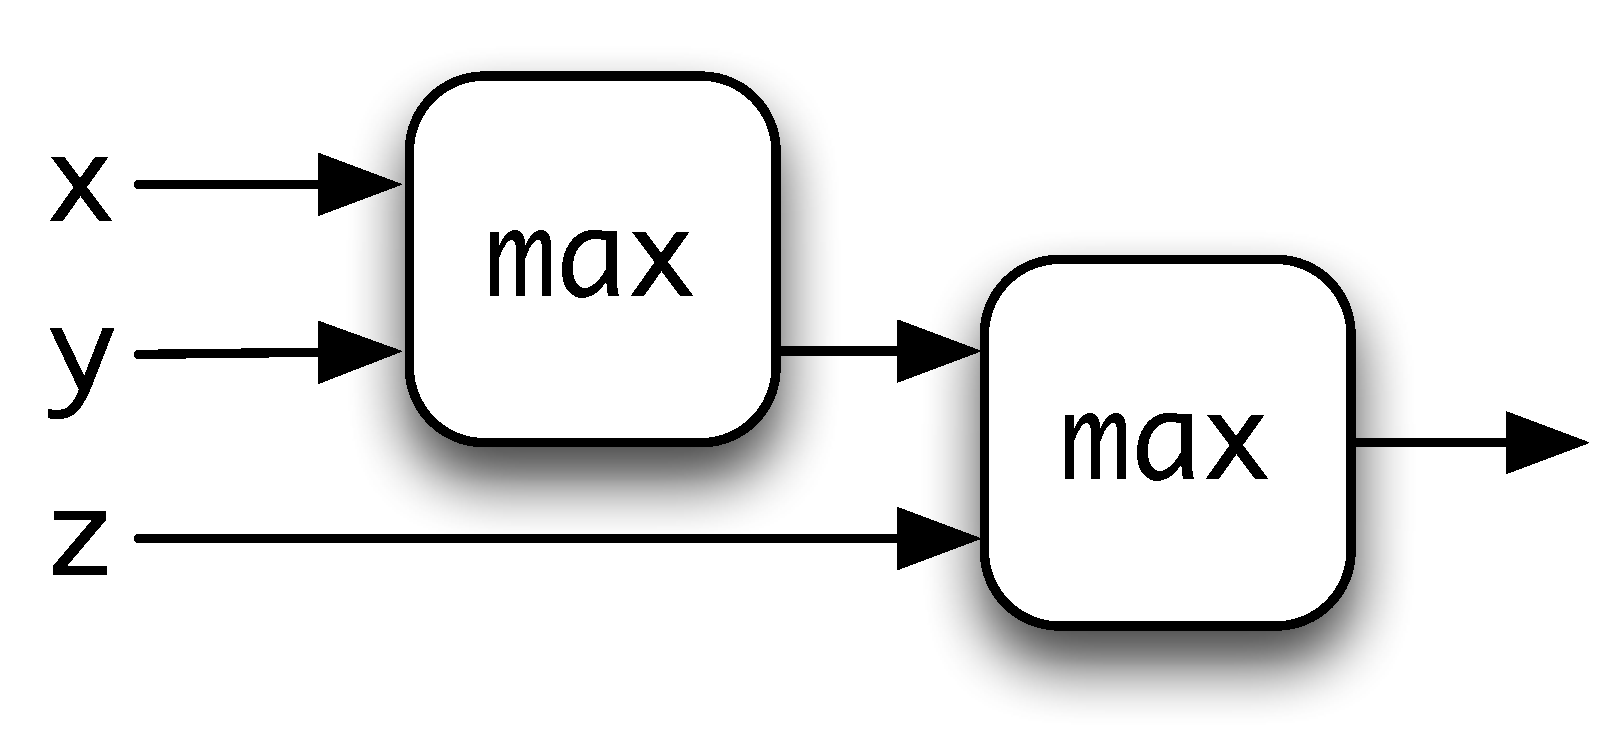
\includegraphics[width=3in]{Pictures/maxThree.pdf}
\end{center} 
and in Haskell
\begin{alltt}
maxThree x y z = max (max x y) z
\end{alltt}
or writing the \texttt{max} in its infix form, \texttt{`max`},
\begin{alltt}
maxThree x y z = (x `max` y) `max` z
\end{alltt}
Using \texttt{max} in this way has some advantages. 

The definition of
\texttt{maxThree} is considerably shorter and easier to read than the
original. If at some point we changed the way that \texttt{max} was
calculated -- perhaps making it a built-in function -- then this
definition would get the benefit of the `new' \texttt{max}. This is not
such an advantage in a small example like this, but can be of
considerable benefit in a larger-scale system where we can expect
software to be modified and extended over its lifetime.

\subsection*{Can I break the problem down into simpler parts?}

If we cannot solve a problem as it stands, we can think about breaking it
down into smaller parts. This principle of `divide and conquer'\index{divide and conquer}
\index{design!divide and conquer} is the
basis of all larger-scale programming: we solve aspects of the problem
separately and then put them together to give an overall solution.

How do we decide how to break a problem down into parts? We can think of
solving a simpler problem and then building the full solution on top, or
we can ask ourselves the question here.

\subsubsection*{{\bfseries What if\/} I had any functions I wanted: which could I use in
writing the solution?} 
\index{design!what if?}

This {\em what if \ldots?\/} is a central question, because it breaks the problem into two
parts. First we have to give the solution {\em assuming\/} we are
given the auxiliary functions we want and thus without worrying about how they are
to be defined. Then, we have separately to define these
auxiliary functions. 
\begin{center}
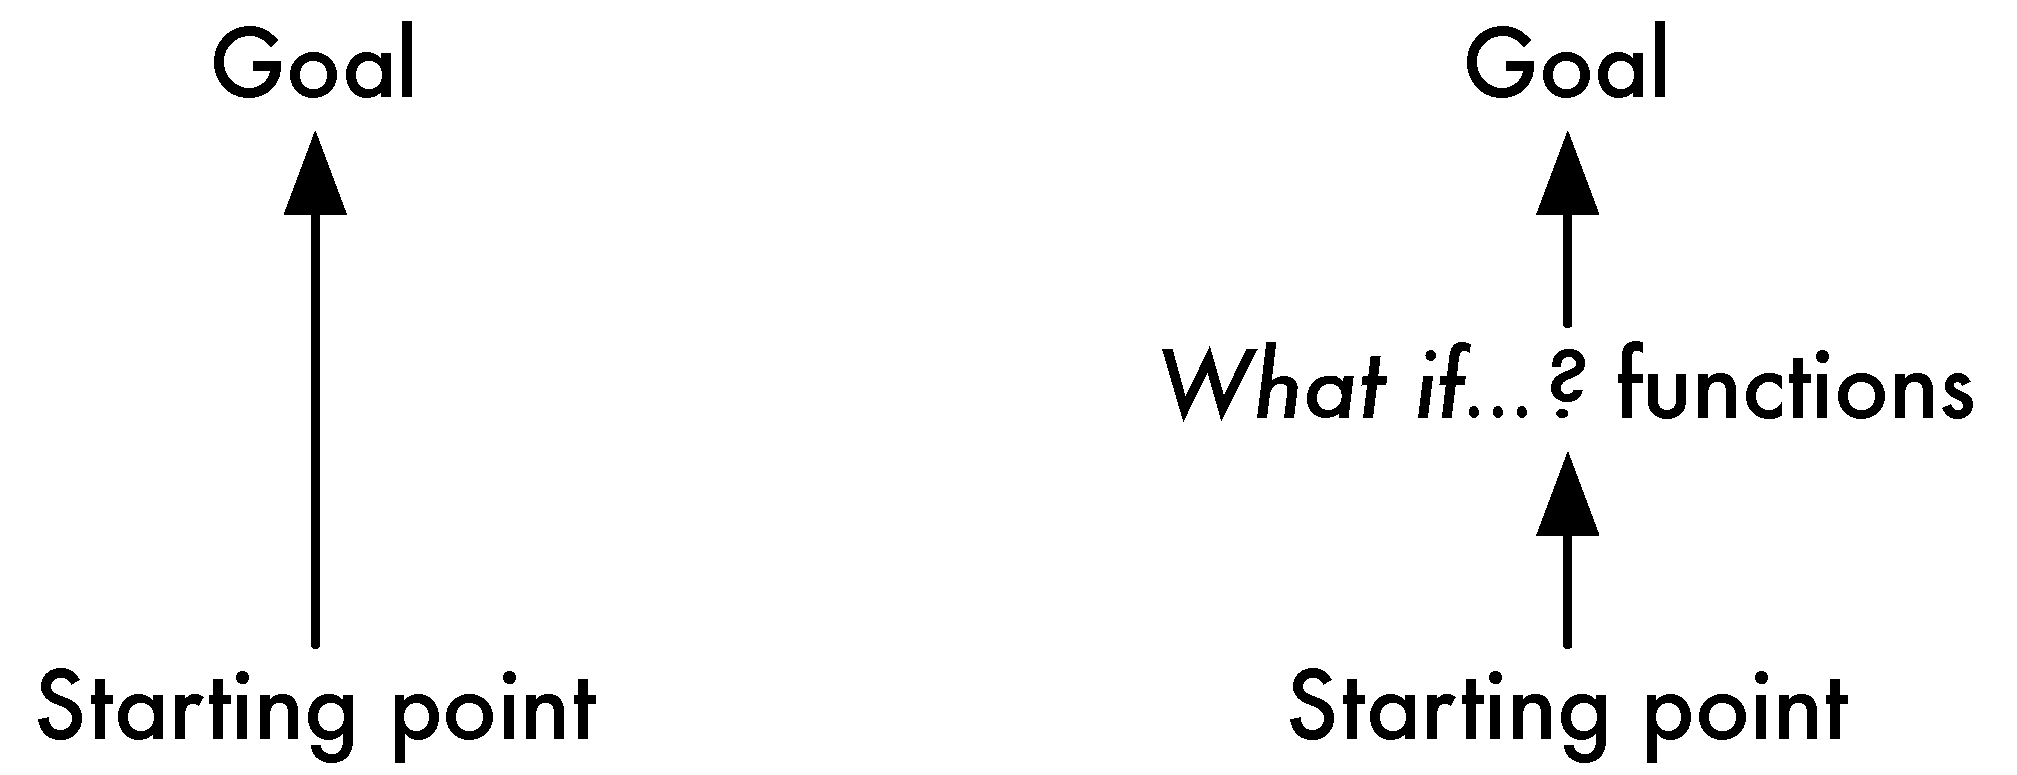
\includegraphics[width=3.5in]{Pictures/whatIf.pdf}
\end{center}
Instead of a single jump from the starting point to the goal, we have
two shorter jumps, each of which should be
easier to do. This approach is called \textbf{top-down}\index{design!top-down}
as we start at the top with the overall problem, and work by breaking it down into smaller
problems. 

This process can be done repeatedly, so that the overall problem is solved in a series
of small jumps.\index{design!iterative} We now look at an example; more examples appear in the exercises at the end
of the section.

Suppose we are faced with the problem of defining
\begin{alltt}\minx{middleNumber}
middleNumber :: Integer -> Integer -> Integer -> Integer 
\end{alltt}
according to the first of the alternatives described on page
\pageref{middleNumb}. A model is given by the definition of
\texttt{maxThree}, in which we give conditions for \texttt{x} to be the
solution, \texttt{y} to be the solution and so on. We can therefore
sketch out our solution like this
\begin{alltt}
middleNumber x y z
  | condition for x to be solution      = x
  | condition for y to be solution      = y
  ....
\end{alltt}
Now, the problem comes in writing down the conditions, but here we say
{\em what if\/} we had a function to do this. Let us call it
\texttt{between}. It has three numbers as arguments, and a Boolean
result, 
\begin{alltt}\minx{between}
between :: Integer -> Integer -> Integer -> Bool
\end{alltt}
and is defined so that \texttt{between m n p} is \texttt{True} if \texttt{n} is
between \texttt{m} and \texttt{p}. We can complete the definition of
\texttt{middleNumber} now:
\begin{alltt}
middleNumber x y z
  | between y x z      = x
  | between x y z      = y
  | otherwise          = z
\end{alltt}
The definition of the function \texttt{between} is left as an exercise for the reader.

This section has introduced some of the general ideas which can help us
to get started in solving a problem. Obviously, because programming is a creative
activity  there is not going to be a set of rules
which will always lead us mechanically to a solution to a problem. On
the other hand, the questions posed here will get us started, and show
us some of the alternative strategies we can use to plan how we are
going to write a program. 

We'll follow this up in the next section, where we look at another way we can break problems down and solve them in steps. After that we'll take a first look at how to define our own data types in solving problems. We take up the discussion again in Chapter \ref{moreDesign}.

\begin{exercises}

\item
This question is about the function
\begin{alltt}
maxFour :: Integer -> Integer -> Integer -> Integer -> Integer
\end{alltt}
which returns the maximum of four integers. Give three definitions of this
function: the first should be modelled
on that of \texttt{maxThree}, the second should use the function
\texttt{max} and the third should use the functions \texttt{max} and
\texttt{maxThree}. For your second and third solutions give diagrams
to illustrate your answers. Discuss the relative merits of the three
solutions
you have given.

\item
Give a definition of the function 
\begin{alltt}
between :: Integer -> Integer -> Integer -> Bool
\end{alltt}
discussed in this section. The definition should be consistent with what we said
in explaining how \texttt{middleNumber}
works. You also need to think carefully about the different ways that
one number can lie between two others. You might find it useful to
define a function
\begin{alltt}
weakAscendingOrder :: Integer -> Integer -> Integer -> Bool
\end{alltt}
so that \texttt{weakAscendingOrder m n p} is \texttt{True} exactly when
\texttt{m}, \texttt{n} and \texttt{p} are in weak ascending order, that is the sequence
does not go down at any point. An example of such a sequence is 
\texttt{2 3 3}.

\item
Give a definition of the function
\begin{alltt}\minx{howManyEqual}
howManyEqual :: Integer -> Integer -> Integer -> Integer
\end{alltt}
which returns how many of its three arguments are equal, so that
\begin{alltt}
howManyEqual 34 25 36 = 0
howManyEqual 34 25 34 = 2
howManyEqual 34 34 34 = 3
\end{alltt}
Think about what functions you have already seen -- perhaps in the exercises --
which you can use in the solution.

\item
Give a definition of the function
\begin{alltt}
howManyOfFourEqual :: Integer -> Integer -> Integer -> Integer -> Integer
\end{alltt}
which is the analogue of \texttt{howManyEqual} for four numbers. You may
need to think {\em what if \ldots?}.
\index{design!where do I start?|)}
\end{exercises}


\section{Solving a problem in steps: local definitions}
\label{intro-localdefs}\label{localDefs}\index{definition!local|(}

In this section we'll look at a way that we can make \emph{local} definitions as a part of making a function definition: these might be definitions of useful functions, or of values which we can use in defining our answers. We start by looking at some examples, and then discuss some of the details of the \texttt{where} and \texttt{let} constructs.

\subsection*{Examples}

\vspace*{-1cm}
\begin{wrapfigure}[5]{r}{3.5cm}
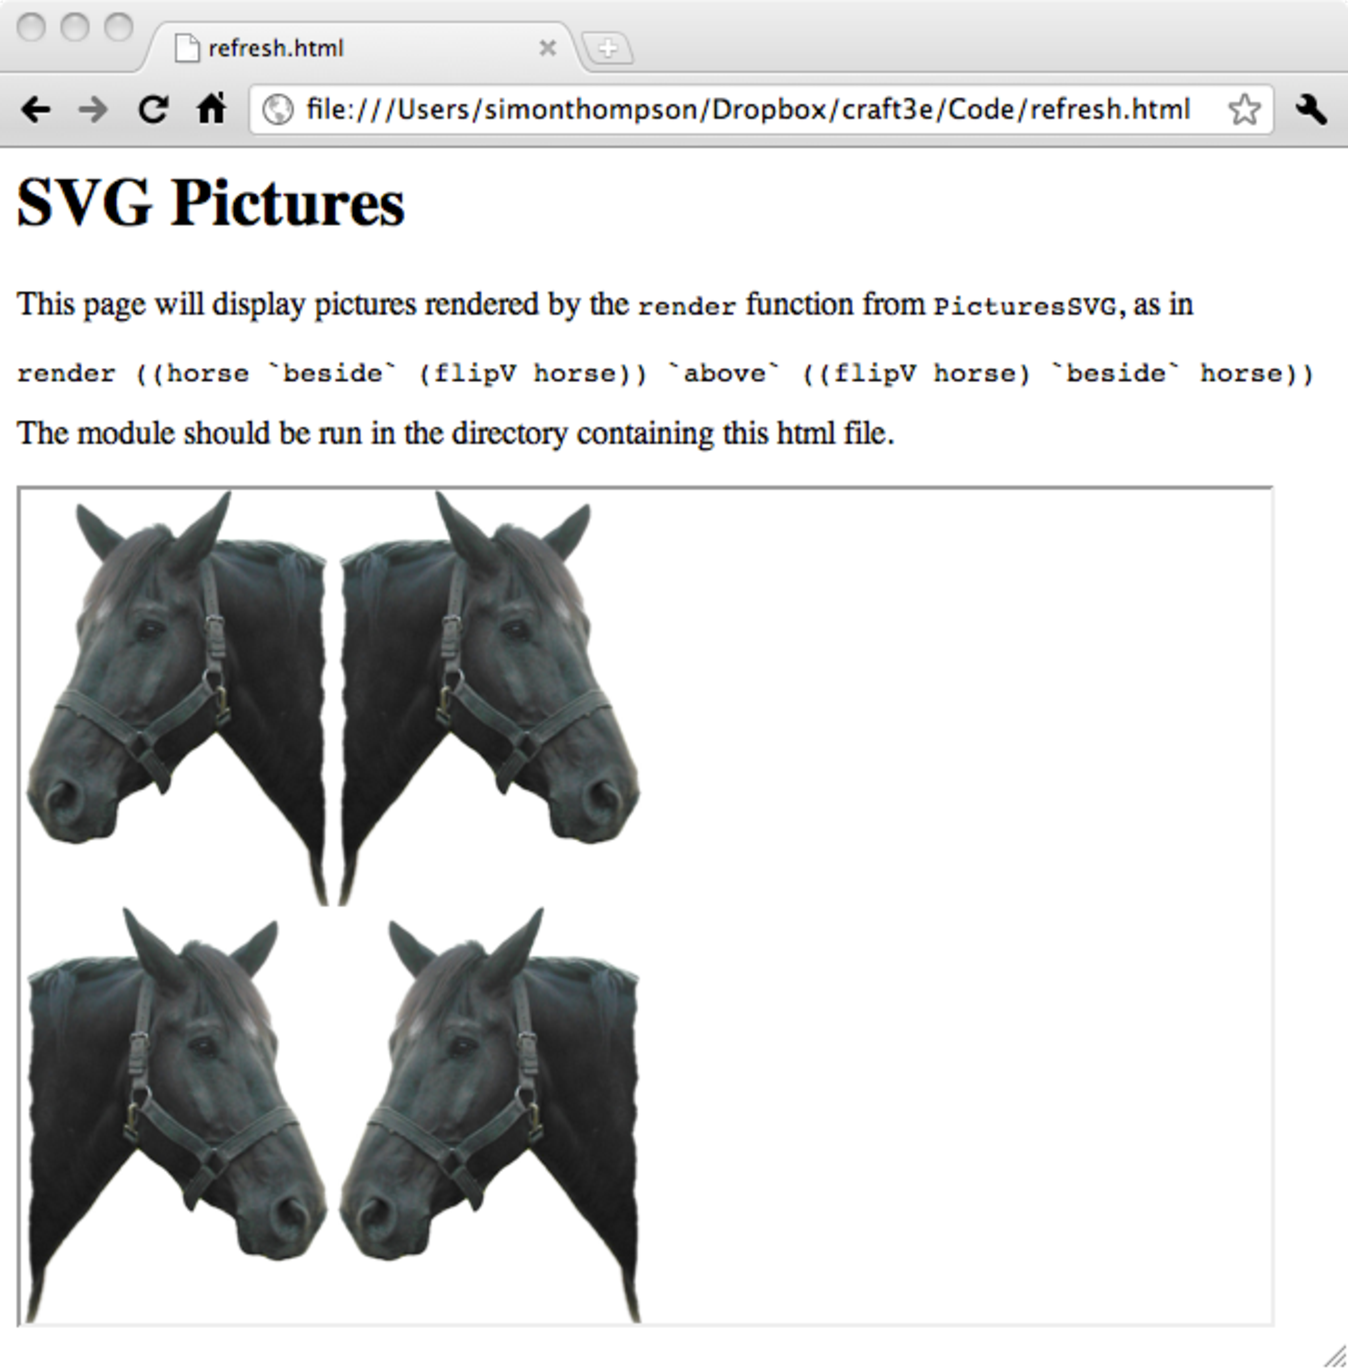
\includegraphics[width=3.5cm]{Pictures/ScreenSVG.pdf}
\end{wrapfigure}
\vspace*{1cm}
The example we will follow is to define a function over pictures, as implemented in the module \texttt{PicturesSVG.hs}. Suppose we want to define a function that takes a picture like horse, and delivers the picture first shown in Figure \ref{svgpix} on page \pageref{svgpix}. 

\medskip
\noindent
One way to tackle it is to start this way:
\begin{alltt}
fourPics :: Picture -> Picture

fourPics pic =
    left `beside` right
      where
        left  = ...
        right = ...
\end{alltt}


\noindent
where we define what \texttt{left} and \texttt{right} mean in the \emph{local definitions} that follow the \texttt{where}. The reason these are called `local' is that they can only be used in the definition of the \texttt{fourPics} function, and nowhere else. 

So, we have broken the problem down into two parts, each simpler than the whole problem. Let's look at the \texttt{left} first. We get this by putting the \texttt{pic} above an inverted version, so giving us
\begin{alltt}\minx{fourPics}\minx{where}
fourPics :: Picture -> Picture

fourPics pic =
    left `beside` right
      where
        left  = pic `above` invertColour pic
        right = ...
\end{alltt}
Now, there are a number of ways of finishing off the definition. Let's look at three of these now.
\begin{itemize}
\item
Let's start by defining \texttt{right} \emph{from scratch}, like this
\begin{alltt}
fourPics :: Picture -> Picture

fourPics pic =
    left `beside` right
      where
        left  = pic `above` invertColour pic
        right = invertColour (flipV pic) `above` flipV pic
\end{alltt}
\item
We could modify this solution so that we \emph{add another local definition} to help us. In this case we define \texttt{flipped} as the original \texttt{pic} flipped in a vertical mirror. We do this because we can use this in defining the right hand side in a similar way to how we defined the left.
\begin{alltt}
fourPics :: Picture -> Picture

fourPics pic =
    left `beside` right
      where
        left    = pic `above` invertColour pic
        right   = invertColour flipped `above` flipped
        flipped = flipV pic
\end{alltt}
\item
We could \emph{use} the definition of \texttt{left} in defining \texttt{right}: we get \texttt{right} from \texttt{left} by reflecting it in a vertical mirror, and then inverting the colour (or the other way around), so giving the definition
\begin{alltt}
fourPics :: Picture -> Picture

fourPics pic =
    left `beside` right
      where
        left  = pic `above` invertColour pic
        right = invertColour (flipV left)
\end{alltt}
\item
Finally, we could  define a \emph{local function}; this is a function we can use only within the definition of \texttt{fourPics}, and not elsewhere. The function \texttt{stack} will put a picture above its inverted version; we'll then use \texttt{stack} in defining the \texttt{left} and \texttt{right} parts of the picture.
\begin{alltt}
fourPics :: Picture -> Picture

fourPics pic =
    left `beside` right
      where
        stack p  = p `above` invertColour p
        left     = stack pic
        right    = stack (invertColour (flipV pic))
\end{alltt}

\end{itemize}
As you can see from this example, there's often more than one way of solving a problem, but a very useful tool in each of these solutions was to use local definitions.

Another more mathematical example is given by a function to calculate the area of a triangle with sides \texttt{a}, \texttt{b} and \texttt{c}. The formula for this is \[\sqrt{\mbox{\texttt{s*(s-a)*(s-b)*(s-c)}}}\]
where \texttt{s} is \texttt{(a+b+c)/2}. As a definition in Haskell this becomes
\begin{alltt}\minx{triArea}
triArea :: Float -> Float -> Float -> Float

triArea a b c 
    | possible   = sqrt(s*(s-a)*(s-b)*(s-c))
    | otherwise  = 0
    where
      s = (a+b+c)/2 
      possible = ... for you to define ...
\end{alltt}
Defining \texttt{possible} is left as an exercise: this value should be \texttt{True} only if it's possible to have a triangle with those sides. Each of the numbers should be positive, and each side should satisfy the \emph{triangle inequality}: the length of the side is less than the sum of the other two sides.


\begin{figure}[t]
\beware{\texttt{let} expressions}{\minx{let}It is also possible to make definitions local to an expression, rather than local to a function clause as for \texttt{where}. For instance,
we can write 
\begin{alltt}
let x = 3+2 in x\^{}2 + 2*x - 4
\end{alltt}
giving the result \texttt{31}. If more than one definition is included in one
line they
need to be separated by semi-colons, thus:
\begin{alltt}\minx{;}
let x = 3+2 ; y = 5-1 in x\^{}2 + 2*x - y
\end{alltt}
We shall find that we use this form only occasionally.}
\end{figure}

\subsection*{Calculation with local definitions}
\index{calculation!local definitions}

We  look at how to calculate with local definitions by taking the example of 
a function which is to
return the sum of the squares of two integers.  
\begin{alltt}
sumSquares :: Integer -> Integer -> Integer\minx{sumSquares}

sumSquares n m 
  = sqN + sqM
    where
    sqN = n*n
    sqM = m*m
\end{alltt}
where the \texttt{where} clause is used to find the two squares.

The way in which calculations are written
can be extended to deal with \texttt{where} clauses. The {\ttfamily
sumSquares} function in the previous section gives, for example
\begin{alltt}
sumSquares 4 3
= sqN + sqM
  where
  sqN = 4*4 = 16
\vertline{30pt}  sqM = 3*3 = 9
= 16 + 9
= 25
\end{alltt}
The values of the local definitions are calculated beneath the \texttt{where} if
their values are needed. All local evaluation below the \texttt{where} is indented. To
follow the top-level value, we just have to look at the calculation at the
left-hand side.

The vertical lines which appear are used to link the successive steps of
a
calculation when these have intermediate \texttt{where} calculations. The lines
can be omitted.

\index{definition!local|)}


\subsection*{Layout}

In definitions with \texttt{where} clauses, the layout is significant. The 
offside rule\index{offside rule} is
used by the 
system to determine the end of each definition in the \texttt{where} clause. 

The \texttt{where} clause
must be found in the definition to which it belongs, so that the \texttt{where}
must occur somewhere to the right of the start of the definition. Inside the
\texttt{where} clause, the same rules apply as at the top level: it is therefore
important that the definitions are aligned vertically -- if not, an error will
result.
Our recommended layout is therefore
\index{layout!recommended}
\index{function definition!layout|see{layout}}
\index{function definition!general form}
\begin{alltt}
f \pone \ptwo ... \pk
  | \gone          = \eone  
   ...
  | otherwise   = \er  
    where
    \vone  \aone ... \subscr{a}{n} = \rone
    \vtwo = \rtwo
    ....
\end{alltt}
The \texttt{where} clause here is attached to the whole of the
conditional equation, and so is attached to all the clauses of the
conditional equation.

This example also shows that the local definitions can include functions
-- here \texttt{\vone} is an example of a local function definition. We have
given type declarations for all top-level definitions; it is
\index{type declaration}
also possible to give type declarations for \texttt{where}-defined objects in
Haskell. In cases where the type of a locally defined object
is not obvious from its context, our convention is to
include a declaration of its type.\index{conventions!local type
declarations}
\vspace{5pt}


\subsection*{Scopes}
\index{scope}

A Haskell script consists of a sequence of definitions. The \textbf{scope} of
a definition is that part of the program in which the definition can be used.
All definitions at the top-level in Haskell have as their scope the whole script that
they are
defined in: that is, they can be used in all the definitions
the script contains. In particular they can be used in definitions
which occur before theirs in the script, as in
\begin{alltt}
isOdd, isEven :: Int -> Bool
\bl
isOdd n 
  | n<=0        = False
  | otherwise   = isEven (n-1)
\bl
isEven n 
  | n<0         = False
  | n==0        = True
  | otherwise   = isOdd (n-1)
\end{alltt}
Local definitions, given by \texttt{where} clauses, are not intended to be
`visible' in the whole of the script, but rather just in the conditional
equation in which
they appear. The same is true of the variables in a function definition:
their scope is the whole of the conditional equation in which they
appear. 

Specifically, in the example which follows, the scope of the
definitions of \texttt{sqx}, \texttt{sqy} and \texttt{sq} and of the variables \texttt{x}
and \texttt{y} is given by the large box; the smaller box gives the scope of the
variable \texttt{z}.
\begin{alltt}
maxsq x y \minx{maxsq}
  \framebox{\begin{minipage}{1in}\begin{tabbing}
\mbox{\ttfamily| sqx > sqy     = sqx}\\
\mbox{\mi| otherwise     = sqy}\\
\rule{0cm}{0.4cm}
\ttfamily    where\\
\ttfamily    sqx  = \mbox{\texttt{sq x}}\\
\ttfamily    sqy  = \mbox{\texttt{sq y}}\\
\rule{0cm}{0.4cm}
\ttfamily    sq :: Int -> Int\\
\ttfamily    sq z = \framebox{\texttt{z*z}}
\end{tabbing}
\end{minipage}
}
\bl
\end{alltt}
In particular it is important to see that
\begin{titemize}
\item the variables appearing on the left-hand side of the function 
definition --
\texttt{x} and \texttt{y} in this case -- can be used in the local definitions; here they are
used in \texttt{sqx} and \texttt{sqy}; 
\item local definitions can be used before they are defined: \texttt{sq} is used
in \texttt{sqx} here;
\item local definitions can be used in results and in guards as well as in
other local definitions.
\end{titemize}
It is possible for a script to have two definitions or variables with the
same name. In the example below, the variable \texttt{x} appears twice. Which
definition is in force at each point? The {\em most local\/} is the one which
is used. 
\index{scope!nested}
\begin{alltt}
maxsq x y 
  \framebox{\begin{minipage}{1in}\begin{tabbing}
\mbox{\ttfamily| sq x > sq y   = sq x}\\
\mbox{\ttfamily| otherwise     = sq y}\\
\rule{0cm}{0.4cm}
\ttfamily    where\\
\rule{0cm}{0.4cm}
\ttfamily    sq x = \framebox{\texttt{x*x}}
\end{tabbing}
\end{minipage}
}
\bl
\end{alltt}
In the example, we can think of the inner box {\em cutting a hole\/} in the
outer, so that the scope of the outer \texttt{x} will exclude the 
definition of \texttt{sq}. When one
definition is contained inside another the best advice is that different
variables and names should be used for the inner definitions unless there is a
very good reason for using the same name twice.

Finally note that it is not possible to have multiple definitions of the
same name at the same level; one of them needs to be hidden if a clash
occurs due to the combination of a number of modules.


\begin{exercises}

\item
Give two other ways of completing the definition of \texttt{fourPics} given in this section.

\item
Another way of solving the problem is to break it down into one picture above another, as in
\begin{alltt}
fourPics :: Picture -> Picture

fourPics pic =
    top `above` bottom
      where
        top    = ...
        bottom = ...
\end{alltt}
Give three different ways of completing this definition.

\item
Give two other ways of defining the \texttt{fourPics} function.

\item
Define the \texttt{possible} value as used in the \texttt{triArea} function.



\item 
Define the function
\begin{alltt}
maxThreeOccurs :: Int -> Int -> Int -> (Int,Int)
\end{alltt}
which returns the maximum of three integers paired with the number of times
it occurs among the three.
A natural solution first finds the maximum, and then investigates how often
it occurs among the three. Discuss how you would write your solution if
you were not allowed to use \texttt{where}-definitions.

\item
Give sample calculations of 
\begin{alltt}
maxThreeOccurs 4 5 5
maxThreeOccurs 4 5 4
\end{alltt}
using your definition of \texttt{maxThreeOccurs} from the previous
question.

\end{exercises}


\section{Defining types for ourselves: enumerated types}
\label{EnumTypes}\index{enumerated type|(}\index{type!enumerated|(}

Often the first thing we need to do in solving a problem is to find the right types to model the problem domain. While Haskell comes with a comprehensive set of basic data types, which we discussed in Chapter \ref{BasicTypes}, and ways of building complex types from simpler ones, which we'll discuss in the coming chapters, it also makes sense to define types which directly model the problem domain. This is done with Haskell \texttt{data} types: this section introduces the simplest cases of these types in the context of a gaming example. 


\subsection*{Rock - Paper - Scissors}\index{Rock - Paper - Scissors|(}\index{RPS|see{Rock - Paper - Scissors}}

\begin{wrapfigure}[8]{r}{5cm}
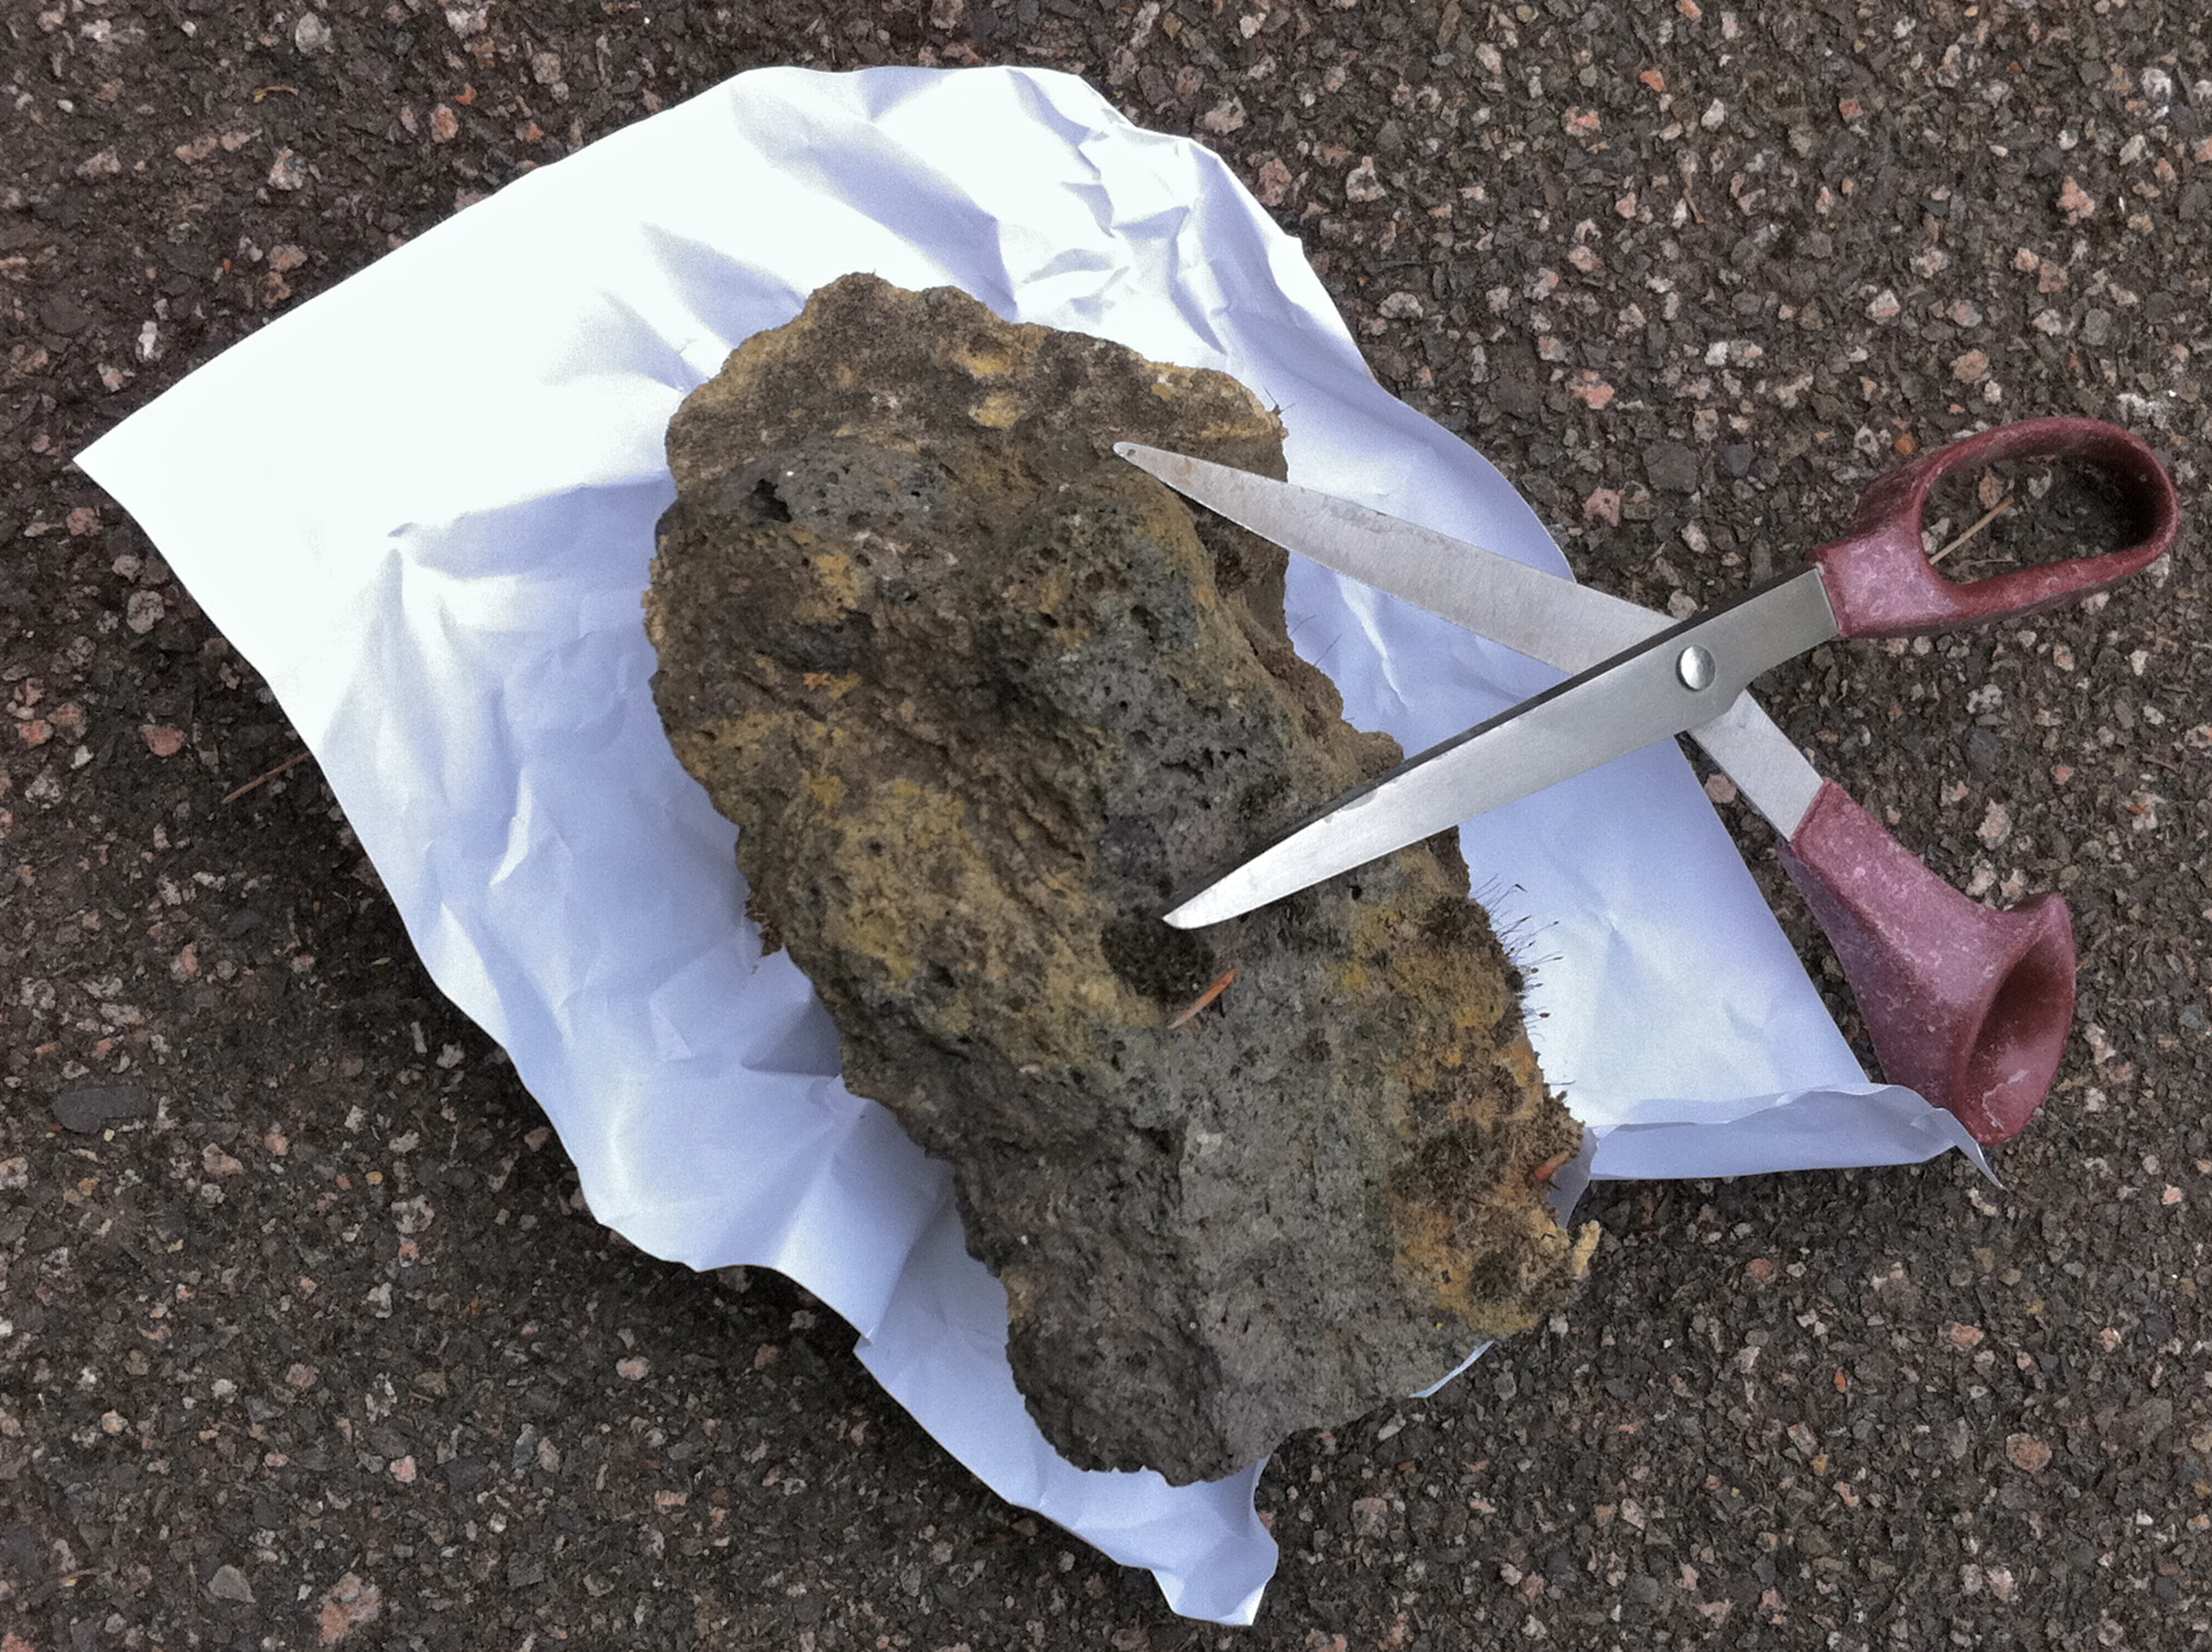
\includegraphics[width=5cm]{Pictures/RPS.pdf}
\end{wrapfigure}
Two players choose one of Rock, Paper and Scissors after counting to three and making one of these gestures:
\begin{itemize}
\item
\textbf{A clenched fist} which represents a rock.
\item
\textbf{A flat hand} representing a piece of paper.
\item
\textbf{Index and middle figure extended} which represents a pair of scissors.
\end{itemize}

\noindent
If they choose the same gesture, neither wins; if not, the result is decided this way:

\begin{itemize}
\item Rock defeats scissors, because a rock will blunt a pair of scissors.
\item Paper defeats rock, because a paper can wrap up a rock.
\item Scissors defeat paper, because scissors cut paper.
\end{itemize}
Suppose that we want to model this in Haskell. One option would be to use integers, characters or strings (which we'll find out about later), but none of these is ideal, for a number of reasons.
\begin{itemize}
\item
A choice may well be arbitrary: what numbers should we associate with `rock', which with `scissors'?
\item
The type we would choose would have lots of other elements which don't correspond to anything in the game.
\end{itemize} 
So, instead, we will define a \texttt{data} type with three members  
\begin{alltt}\minx{Move}
data Move = Rock | Paper | Scissors
\end{alltt}
where we list the members separated by a vertical bar. We can also put the different members on different lines, like this:
\begin{alltt}
data Move = Rock | 
            Paper | 
            Scissors
\end{alltt}
Whatever the case, we add another line -- some `Haskell magic' which we'll explain in Chapter \ref{typeClasses} -- which allows us to compare elements of this type for equality, and also to be able to see them printed out (or `shown'), like so:
\begin{alltt}\minx{deriving}
data Move = Rock | Paper | Scissors
            deriving (Show,Eq)
\end{alltt}
Now we can begin to define functions using the \texttt{Move} type.
Let's write a function which tells us the move to \texttt{beat} a particular move:
\begin{alltt}\minx{beat}
beat :: Move -> Move

beat Rock     = Paper
beat Paper    = Scissors
beat Scissors = Rock
\end{alltt}
and also the move that will \texttt{lose} against a particular move.
\begin{alltt}\minx{lose}
lose :: Move -> Move

lose Rock  = Scissors
lose Paper = Rock
lose _     = Paper
\end{alltt}
In the definition of \texttt{lose} we've used a wildcard `\_' instead of \texttt{Scissors} in the final clause of the definition. That is because this clause is only matched when the others don't, and that will only happen for the value \texttt{Scissors}.

We will come back to this example in Section \ref{strategiesRPS} once we have covered lists in Haskell, when we'll 
look at some of the strategies for playing (and winning!) Rock - Paper - Scissors.


\begin{exercises}

\item
Define a \texttt{data} type \texttt{Result} which represents the outcome of a round of rock - paper - scissors, which will either be a win. lose or draw.

\item
Define a function
\begin{alltt}
outcome :: Move -> Move -> Result
\end{alltt}
so that this gives the outcome of a round for the first player. For example, we should expect that \texttt{outcome Rock Scissors} should be a win.

\item
We have added some `magic' to the \texttt{Chapter4} module to allow QuickCheck properties to be tested over the \texttt{Move} type. Define a QuickCheck property which connects the results of \texttt{beat} and \texttt{lose}.

\item
How would you define a QuickCheck property to test the \texttt{outcome} function?

\end{exercises}

\subsection*{Standard types}

We can see some standard types as being defined in this way. In particular, we could define \texttt{Bool} like this:
\begin{alltt}\minx{Bool}
data Bool = False | True
            deriving (Show, Eq, Ord)
\end{alltt}
Deriving \texttt{Ord} means that the elements have an ordering defined on them; in this case \texttt{False < True}.

\begin{exercises}

\item
Define a type of seasons, \texttt{Season}, and give a function from seasons to temperature given by the type
\begin{alltt}
data Temp = Cold | Hot
            deriving (Eq, Show, Ord)
\end{alltt}
In defining this function assume that you're in the UK.

\item
Define a type \texttt{Month} and a function from this type to \texttt{Season}, assuming that you're in the northern hemisphere.

\end{exercises}

\index{Rock - Paper - Scissors|)}
\index{enumerated type|)}\index{type!enumerated|)}

\section{Recursion}
\label{recursionIntro}
\index{recursion|(}

Recursion is an important programming mechanism, in which a definition of
a function or other object refers to the object itself. This section
concentrates on explaining the idea of recursion, and why it makes
sense.
In particular we give two complementary explanations
of how primitive recursion works in defining the factorial function over the
natural numbers. In the section after this we look at how recursion is
{\em used\/} in practice.

\subsection*{Getting started: a story about factorials}
\index{factorial|(}
\index{recursion!justification|(}

Suppose that someone tells us that the factorial of a natural number is
the product of all natural numbers from one up to (and including) that number, so
that, for instance
\begin{alltt}
fac 6 = 1*2*3*4*5*6
\end{alltt}
Suppose we are also asked to write down a table of factorials, 
where we take the factorial of zero to be
one. We begin thus
\begin{alltt}
  n      fac n
  0        1
  1        1 
  2        1*2 = 2
  3        1*2*3 = 6
  4        1*2*3*4 = 24
\end{alltt}
but we notice that we are repeating a lot of multiplication in doing
this. In working out
\begin{alltt}
1*2*3*4
\end{alltt} we see that we are repeating the
multiplication of \texttt{1*2*3} before multiplying the result by
\texttt{4}
\begin{alltt}
\framebox{1*2*3}\hspace{3pt}*4
\end{alltt}
and this suggests that we can produce the table in a different way, by
saying how to start
\begin{alltt}
fac 0 = 1\hfill(fac.1)
\end{alltt}
which starts the table thus
\begin{alltt}
  n      fac n
  0        1
\end{alltt}
and then by saying how to go from one line to the next
\begin{alltt}
fac n = fac (n-1) * n\hfill(fac.2)
\end{alltt}
since this gives us the lines
\begin{alltt}
  n      fac n
  0        1
  1        1*1 = 1
  2        1*2 = 2
  3        2*3 = 6
  4        6*4 = 24
\end{alltt}
and so on.

What is the moral of this story? We started off describing the table in
one way, but came to see that all we needed was the information in
\texttt{(fac.1)} and \texttt{(fac.2)}.
\begin{itemize}
\item \texttt{(fac.1)} tells us the first line of the table, and
\item \texttt{(fac.2)} tells us how to get from one line of the table to
the next.
\end{itemize}
The table is just a written form of the factorial function, so we can
see that
\texttt{(fac.1)} and \texttt{(fac.2)}
actually describe the \textbf{function} to calculate the factorial, and
putting them together we get
\begin{alltt}\minx{fac}
fac :: Integer -> Integer
fac n
  | n==0        = 1
  | n>0         = fac (n-1) * n
\end{alltt}
A definition like this is called \textbf{recursive} because we actually
use \texttt{fac} in describing \texttt{fac}
itself. Put this way it may sound paradoxical: after all,
how can we describe something in
terms of itself? But, the story we have just told shows that the definition
is perfectly sensible, since it gives
\begin{itemize}
\item a starting point: the value of \texttt{fac} at \texttt{0}, and
\item a way of going from the value of \texttt{fac} at a particular
point, \texttt{fac (n-1)}, to the value of \texttt{fac} on the next
line, namely \texttt{fac n}.
\end{itemize}
These recursive rules will give a value to \texttt{fac n} whatever the
(positive) value \texttt{n}
has -- we just have to write out \texttt{n}
lines of the table, as it were.


\subsection*{Recursion and calculation}
\index{calculation!and recursion}
\index{recursion!and calculation}

The story in the previous section described how the definition of factorial
\begin{alltt}
fac :: Integer -> Integer
fac n
  | n==0        = 1\hfill(fac.1)
  | n>0         = fac (n-1) * n\hfill(fac.2)
\end{alltt}
can be seen as generating the table of factorials, starting from \texttt{fac
0} and working up to \texttt{fac 1}, \texttt{fac 2} and so forth, up to
any value we wish.

We can also read the definition in a calculational way, and see
recursion justified in another way. Take the example of \texttt{fac 4}
\begin{alltt}
fac 4
\step fac 3 * 4
\end{alltt}
so that \texttt{(fac.2)} replaces one goal -- \texttt{fac 4} -- with a
simpler goal -- finding \texttt{fac 3} (and multiplying it by
\texttt{4}). Continuing to use \texttt{(fac.2)}, we have
\begin{alltt}
fac 4
\step fac 3 * 4
\step (fac 2 * 3) * 4
\step ((fac 1 * 2) * 3) * 4
\step (((fac 0 * 1) * 2) * 3) * 4
\end{alltt}
Now, we have got down to the simplest case (or \textbf{base case}),
\index{recursion!base case}
which is solved by \texttt{(fac.1)}.
\begin{alltt}
\step (((1 * 1) * 2) * 3) * 4
\step ((1 * 2) * 3) * 4
\step (2 * 3) * 4
\step 6 * 4
\step 24
\end{alltt}
In the calculation we have worked from the goal back down to the base
case, using the \textbf{recursion step}
\index{recursion!recursion step}
 \texttt{(fac.2)}. We can again
see that we get the result we want, because the recursion step takes us
from a more complicated case to a simpler one, and we have given a value
for the simplest case (zero, here) which we will eventually reach.

We have now seen in the case of \texttt{fac} two explanations for why
recursion works. 
\begin{itemize}
\item\index{recursion!bottom-up}
The \textbf{bottom-up} explanation says that the \texttt{fac} equations can be 
seen to generate the
values of \texttt{fac} one-by-one from the base case at zero. 
\item\index{recursion!top-down}
A \textbf{top-down} view starts with a goal to be evaluated, and shows how
the equations simplify this until we hit the base case.
\end{itemize}
The two views here are related, since we can think of the top-down
explanation generating a table too, but in this case the table is
generated as it is needed. Starting with the goal of \texttt{fac 4} we
require the lines for \texttt{0} to \texttt{3} also.

Technically, we call the form of recursion we have seen here
\textbf{primitive recursion}.\index{recursion!primitive}
\index{primitive recursion} We will describe it more formally in the
next section, where we examine how to start to find recursive
definitions. Before we do that, we discuss another aspect of the
\texttt{fac} function as defined here.
\index{factorial|)}
\index{recursion!justification|)}

\subsection*{Undefined or error values}
\index{undefinedness}
\index{value!undefined}
\index{value!error}

Our definition of factorial covers zero and the positive integers. What
will be the effect of applying \texttt{fac}
to a negative number? On evaluating \texttt{fac (-2)} in GHCi we receive
the error message
\begin{alltt}
*** Exception: Chapter4.hs:(106,0)-(108,33): 
        Non-exhaustive patterns in function fac
\end{alltt}
because \texttt{fac} is not defined on the negative numbers, since the patterns in the definition of \texttt{fac} don't cover the case of negative numbers.

We could if
we wished extend the definition to zero, on the negative numbers, thus
\begin{alltt}
fac n
  | n==0        = 1
  | n>0         = fac (n-1) * n
  | otherwise   = 0
\end{alltt}
or we could include our own error message, as follows
\begin{alltt}
fac n
  | n==0        = 1
  | n>0         = fac (n-1) * n
  | otherwise   = error "fac only defined on natural numbers"\minx{error}
\end{alltt}
so that when we evaluate \texttt{fac (-2)} we receive the message
\begin{alltt}
Program error: fac only defined on natural numbers
\end{alltt}
The error message here is a Haskell string, as discussed in Chapter
5.

\begin{exercises}

\item Define the function \texttt{rangeProduct}
which when given natural numbers \texttt{m} and
\texttt{n} returns the product 
\begin{alltt}
m*(m+1)*...*(n-1)*n
\end{alltt}
You should include in your definition the type of the function, and your function
should return \texttt{0} when \texttt{n} is smaller than \texttt{m}.\\
{Hint:} you do
not need to use recursion in your definition, but you may if you wish.

\item As \texttt{fac} is a special case of \texttt{rangeProduct}, 
write a definition of \texttt{fac}
which {\em uses\/} \texttt{rangeProduct}.
\end{exercises}

\section{Primitive recursion in practice}

This section examines how primitive recursion is used in practice by
examining a number of examples.

The pattern of primitive recursion says that we can define a function
from the natural numbers \texttt{0}, \texttt{1}, \ldots by giving the
value at zero, and by explaining how to go from the value at
\texttt{n-1} to the value at \texttt{n}. We can give a \textbf{template} for this
\begin{alltt}\index{primitive recursion!template}
fun n
  | n==0        = ....\hfill(prim)
  | n>0         = .... fun (n-1) ....
\end{alltt}
where we have to supply the two right-hand sides.

How can we decide whether a function can be defined in this way? Just as we did
earlier in the chapter, we frame a question which summarizes the
essential property we need for 
primitive recursion to apply.

\subsubsection*{{\bfseries What if\/} we were given the value 
{\tt fun} {\tt (n-1)}. How could we define {\tt fun} {\tt n\/} from it?}

We see how this form of recursion works in practice by looking at some examples.
\index{primitive recursion!examples on numbers}

\begin{example} 
\noindent{\sf 1.}\hskip1em Suppose first that we are asked to
define the function to give us powers of two for natural numbers
\begin{alltt}
power2 :: Integer -> Integer
\end{alltt}
so that \texttt{power2 n} is \superscr{2}{n}, that is \texttt{2}
multiplied by itself \texttt{n} times.
The template is
\begin{alltt}
power2 n
  | n==0        = ....
  | n>0         = .... power2 (n-1) ....
\end{alltt}
In the zero case the result is \texttt{1}, and in general
\superscr{2}{n} is
\superscr{2}{n-1} multiplied by 2, so we define
\begin{alltt}\minx{power2}
power2 n
  | n==0        = 1
  | n>0         = 2 * power2 (n-1)
\end{alltt}

\subexample*{2.}As the next example we take the function
\begin{alltt}\minx{sumFacs}
sumFacs :: Integer -> Integer
\end{alltt}
so that
\begin{alltt}
sumFacs n = fac 0 + fac 1 + ... + fac (n-1) + fac n
\end{alltt}
If we are told that \texttt{sumFacs 4} is \texttt{34} then we can work
out \texttt{sumFacs 5} in one step: we simply add \texttt{fac 5}, that
is \texttt{120}, giving the result \texttt{154}. This works in general, and so 
we can fill in the
template like this:
\begin{alltt}\minx{sumFacs}
sumFacs :: Integer -> Integer
sumFacs n
  | n==0        = 1
  | n>0         = sumFacs (n-1) + fac n  
\end{alltt}
In fact this pattern works for any function \texttt{f} of type 
\texttt{Integer -> Integer} in the place of \texttt{fac}, so
we can say
\begin{alltt}\minx{sumFun}
sumFun :: (Integer -> Integer) -> Integer -> Integer
sumFun f n
  | n==0        = f 0
  | n>0         = sumFun f (n-1) + f n  
\end{alltt}
where the function whose values are being added is itself an argument of the 
\texttt{sumFun}
function.
A sample calculation using \texttt{sumFun} is
\begin{alltt}
sumFun fac 3
\step sumFun fac 2 + fac 3
\step sumFun fac 1 + fac 2 + fac 3
\step sumFun fac 0 + fac 1 + fac 2 + fac 3
\step fac 0 + fac 1 + fac 2 + fac 3
\step ...
\step 10
\end{alltt}
and we can define \texttt{sumFacs} from \texttt{sumFun} thus:
\begin{alltt}
sumFacs n = sumFun fac n
\end{alltt}

We briefly introduced the idea of functions as data
in Chapter \ref{intro}, and we will revisit it in detail in 
Chapter \ref{patternsGen}. As we mentioned in Chapter \ref{intro}, having functions as
arguments is powerful  and \texttt{sumFun}
gives a good example: one definition serves to sum the values of {\em any\/} function 
of type  \texttt{Integer -> Integer} over the range of arguments from \texttt{0} to \texttt{n}. 

\subexample*{3.}As a last example we look at a geometrical
problem. Suppose we want to find out the maximum number of
pieces we can get by making a given number of straight-line
cuts  across a piece of paper. With no cuts we get one piece;
what about the general case? Suppose we have \texttt{n-1} lines
already, and that we add one more. 
\begin{center}
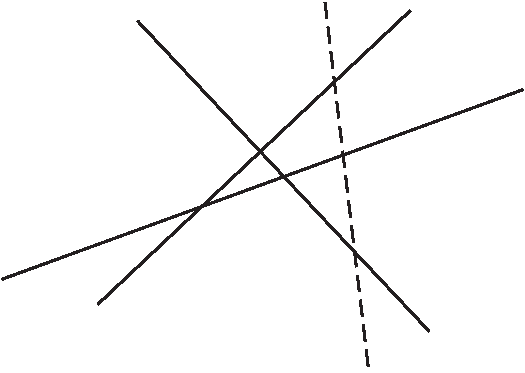
\includegraphics{Pictures/cuts.pdf}
\end{center}
We will get the most new
regions if we cross each of these lines; because they are straight
lines, we can only cut each one once. This means that the new line
crosses exactly \texttt{n} of the regions, and so splits each of these
into two. We therefore get \texttt{n} new regions by adding the
\texttt{n}th line. Our function definition is given by filling in the template 
\texttt{(prim)} according to what we have said.
\begin{alltt}\minx{regions}
regions :: Integer -> Integer 
regions n
  | n==0        = 1
  | n>0         = regions (n-1) + n
\end{alltt}
\end{example}

\begin{exercises}

\item Using the addition function over the natural numbers, give a recursive definition 
of multiplication of natural numbers.

\item The integer square root of a positive integer \texttt{n} is the largest
integer whose square is less than or equal to \texttt{n}. For instance,
the integer square roots of \texttt{15}
and \texttt{16} are \texttt{3} and \texttt{4}, respectively. Give a
primitive recursive definition of this function.

\item Given a function \texttt{f} of type \texttt{Integer -> Integer} give a
recursive definition of a function of type \texttt{Integer -> Integer}
which on input \texttt{n} returns the 
maximum of the values \texttt{f 0}, \texttt{f 1}, \ldots, \texttt{f n}. You
might find the \texttt{max} function defined in Section \ref{guards} useful.

To test this function, add to your script a definition of some values of
\texttt{f} thus:
\begin{alltt}
f 0 = 0
f 1 = 44
f 2 = 17
f _ = 0
\end{alltt}
and so on; then test your function at various values.

\item Given a function \texttt{f} of type \texttt{Integer -> Integer} give a
recursive definition of a function of type \texttt{Integer -> Bool}
which on input \texttt{n} returns \texttt{True} if one or more of the values
\texttt{f 0}, \texttt{f 1}, \ldots, \texttt{f n} is zero and
\texttt{False} otherwise.

\item
Can you give a definition of \texttt{regions}
which instead of being recursive {\em uses\/} the function \texttt{sumFun}?

\item 
{[Harder]} Find
out the maximum number of pieces we can get
by making a given number of flat (that is planar) cuts 
through a solid block. It is {\em not\/} the same answer as we calculated
for straight-line cuts of a flat piece of paper. 
\end{exercises}


\section{Extended exercise: pictures}
\index{pictures!extended exercise|(}

This section looks at how recursion over integers can be used to describe geometrical patterns, using pictures as implemented in \texttt{PicturesSVG} (or \texttt{Pictures}).
We start by giving a definition of a line of \texttt{n} black squares:
\begin{alltt}
blackSquares :: Integer -> Picture

blackSquares n
  | n<=1	     = black
  | otherwise = black `beside` blackSquares (n-1)
\end{alltt}
or diagrammatically,
\begin{center}
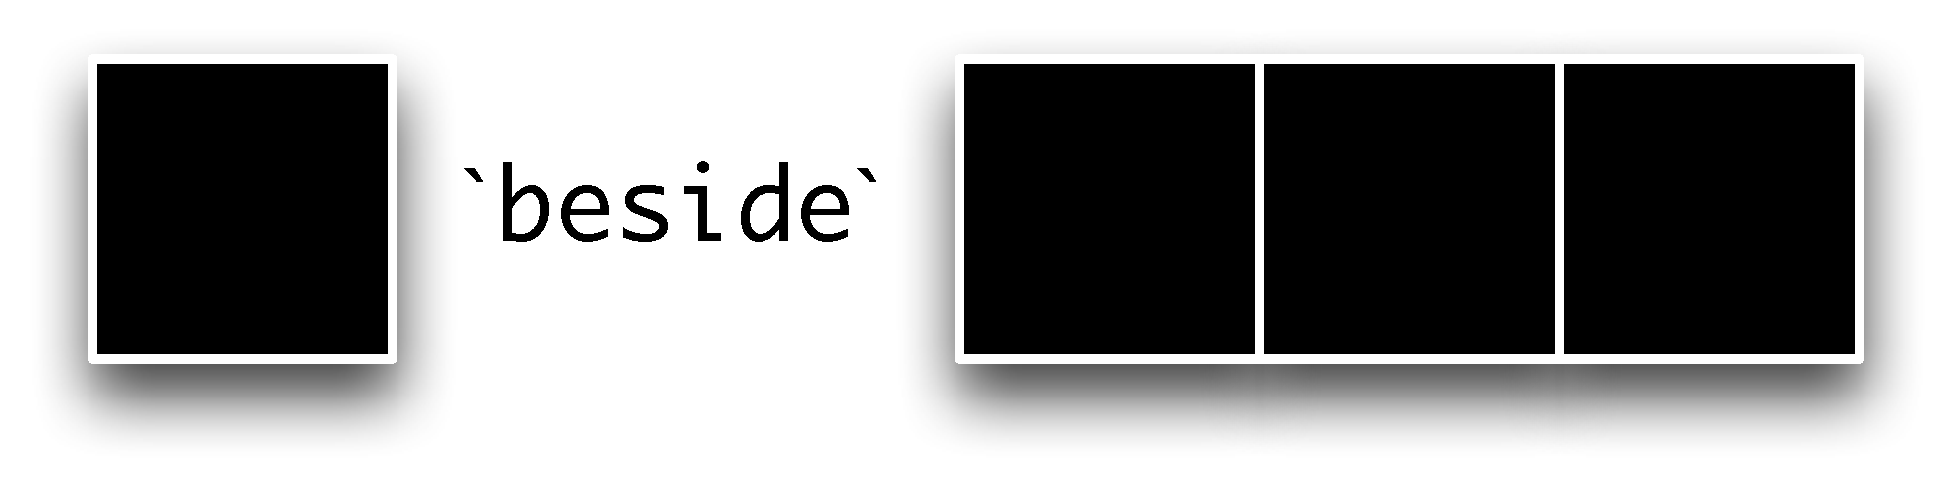
\includegraphics[width=2.5in]{Pictures/blackSquares.pdf}
\end{center}
Suppose that we want to build a line of alternating black and white squares: we get this by putting a black square on the front of a line beginning with a white square:
\begin{alltt}
blackWhite :: Integer -> Picture

blackWhite n
  | n<=1	     = black
  | otherwise = black `beside` whiteBlack (n-1)
\end{alltt}
where \texttt{whiteBlack} is the function that builds a line of alternating squares, beginning with a white. Diagrammatically this is given by
\begin{center}
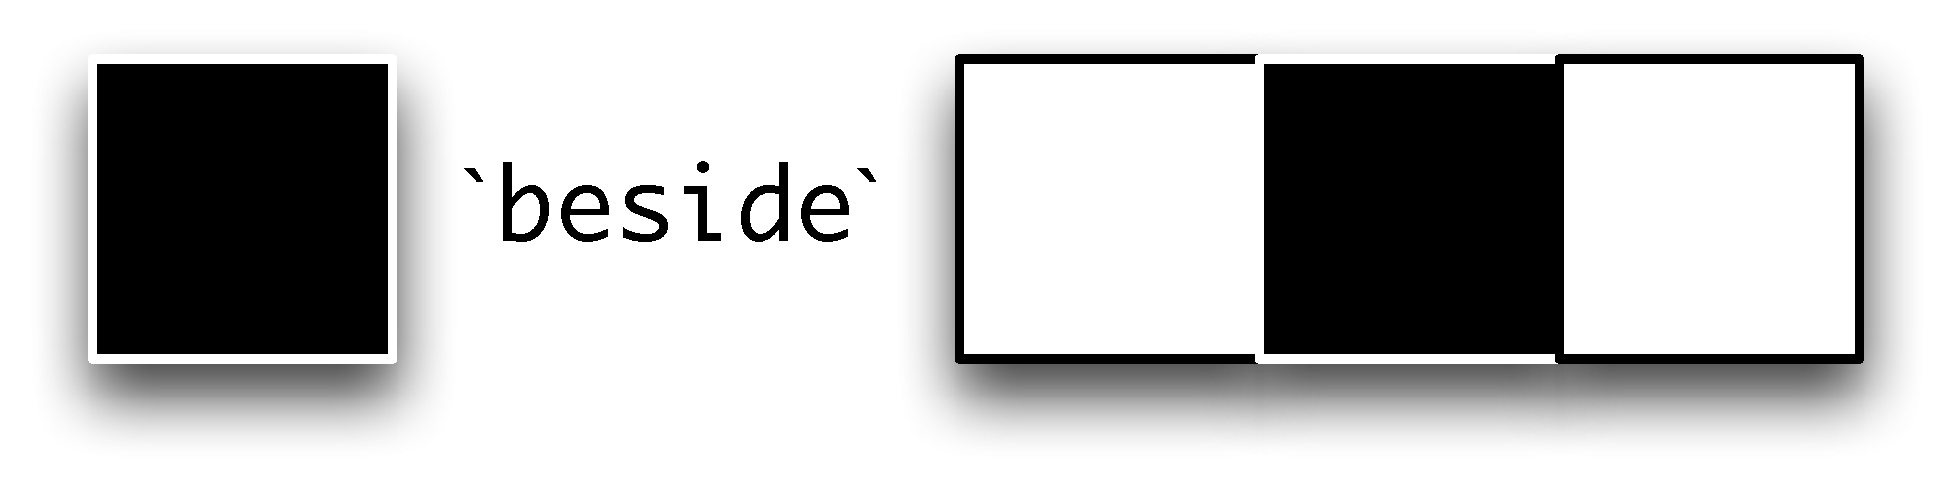
\includegraphics[width=2.5in]{Pictures/blackWhite.pdf}
\end{center}
Using these functions we can build chessboards of any shape:
\begin{alltt}
blackChess :: Integer -> Integer -> Picture

blackChess n m
  | n<=1	     = blackWhite m
  | otherwise = blackWhite m `above` whiteChess (n-1) m
\end{alltt}
where the corresponding function \texttt{whiteChess} builds a board with a white square in the top left-hand corner. Diagrammatically,
\begin{center}
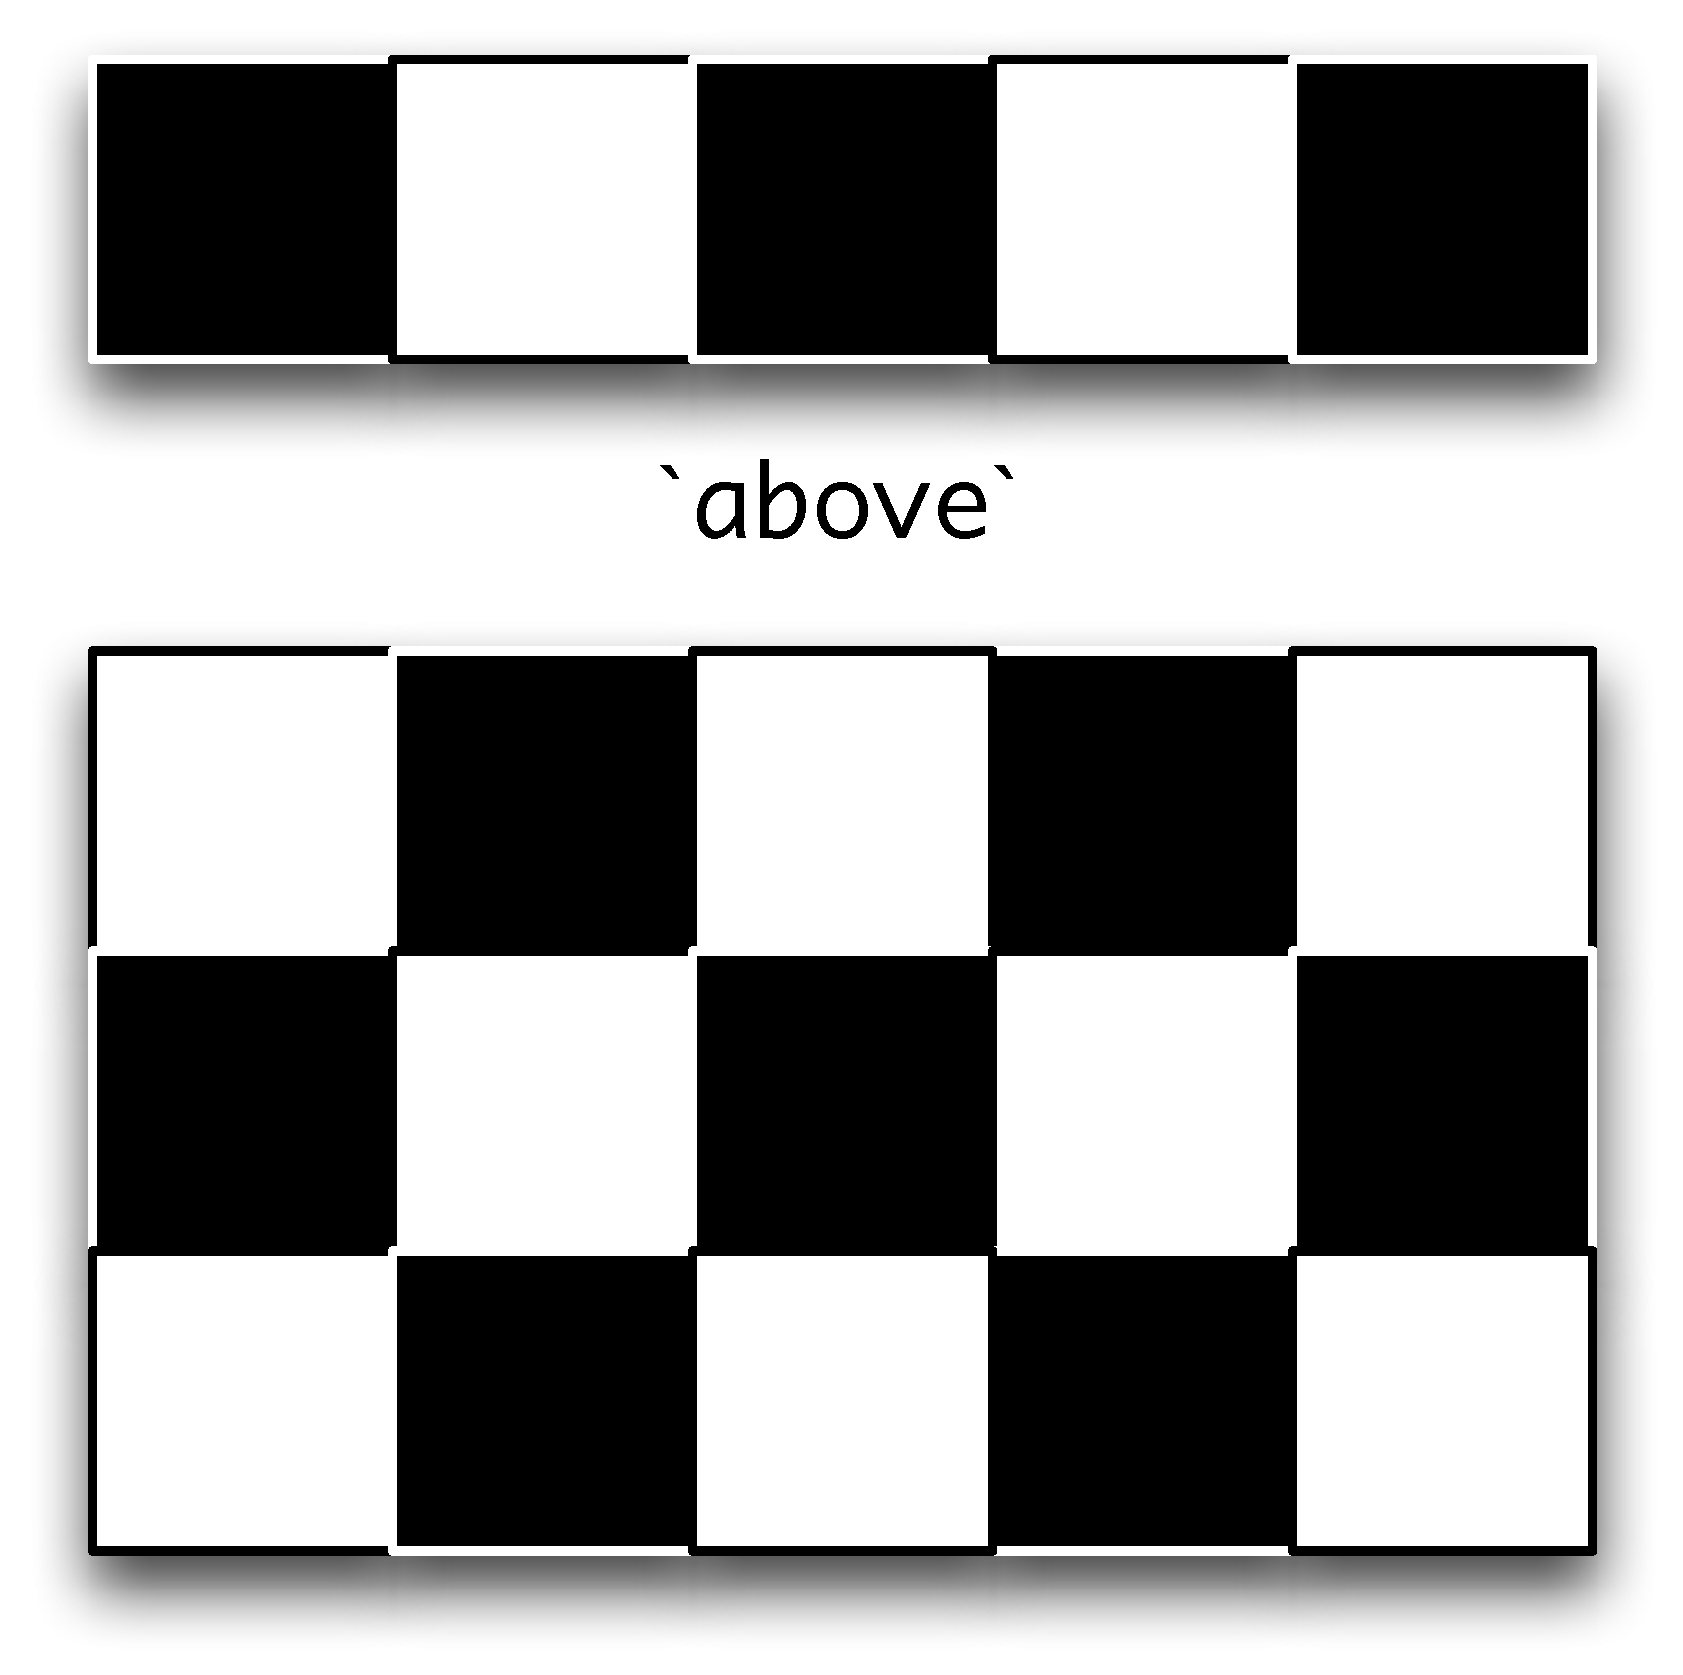
\includegraphics[width=2.5in]{Pictures/chess4.pdf}
\end{center}

\begin{wrapfigure}[8]{r}{1cm}
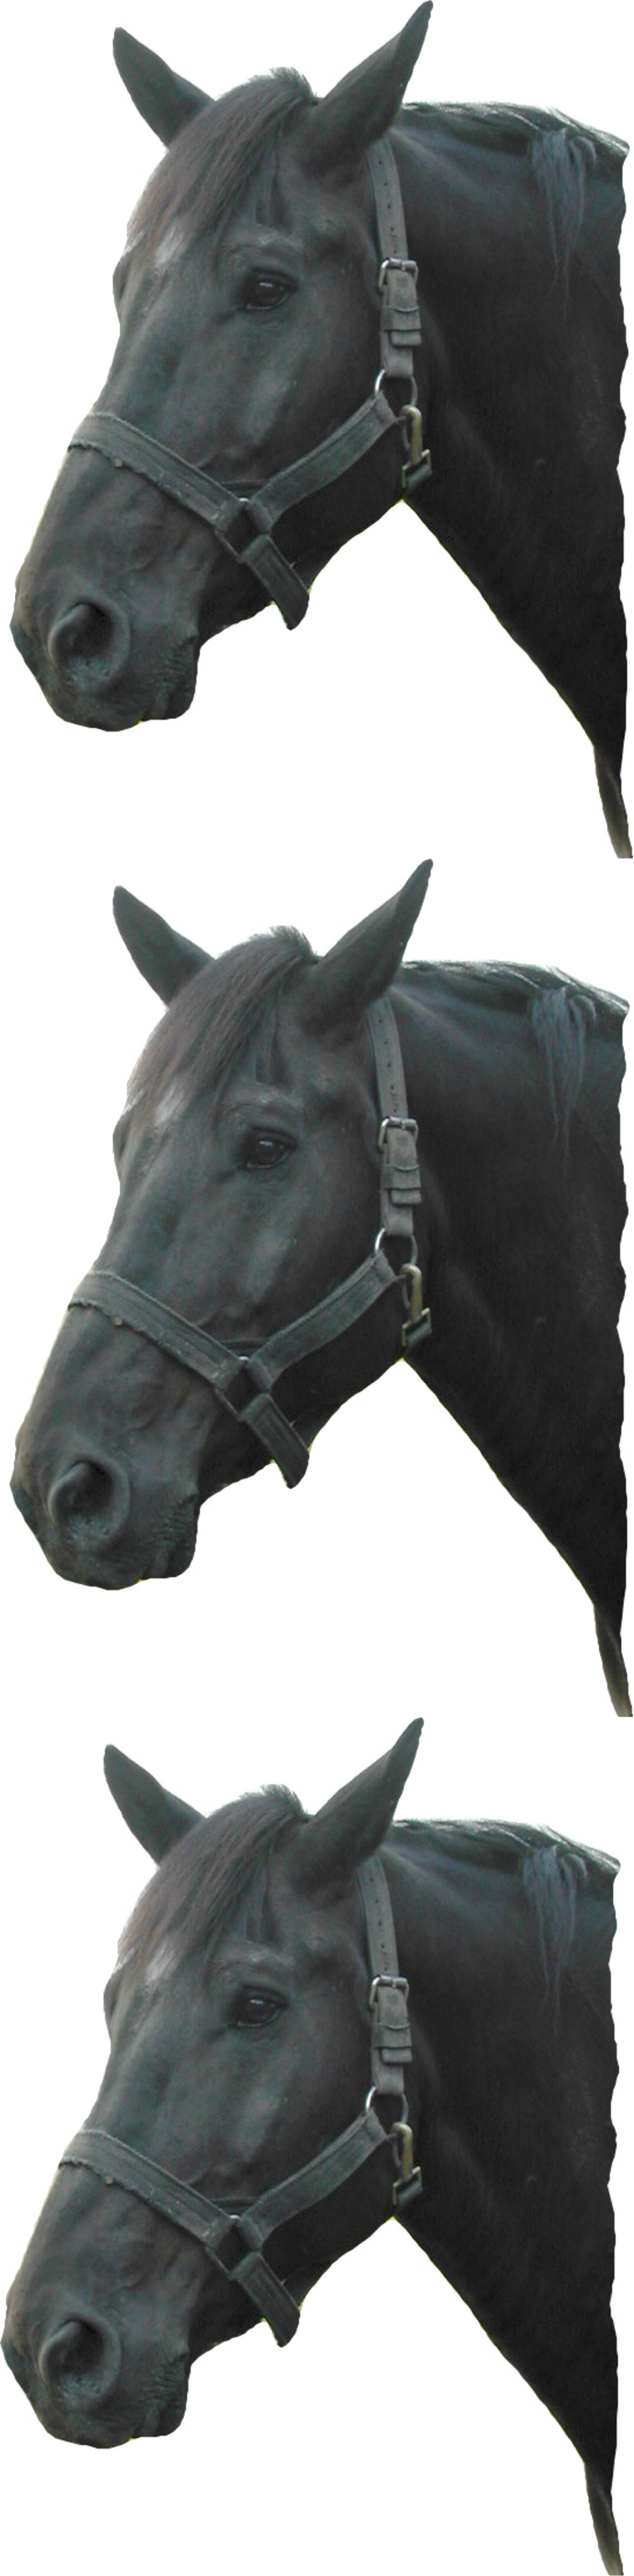
\includegraphics[width=1cm]{Pictures/threeHorses.pdf}
\end{wrapfigure}

\begin{exercises}

\item
Complete the definitions of \texttt{whiteBlack} and \texttt{whiteChess}.

\item
How would you define a function to give a column of pictures,
\begin{alltt}
column :: Picture -> Integer -> Picture
\end{alltt}
so that the result of \texttt{\ column horse 3\ } is as shown to the right.

\item
Give a Haskell function which takes an integer \texttt{n} and returns an  \texttt{n} by \texttt{n} white square with a diagonal black line from top left to bottom right, as in.
\begin{center}
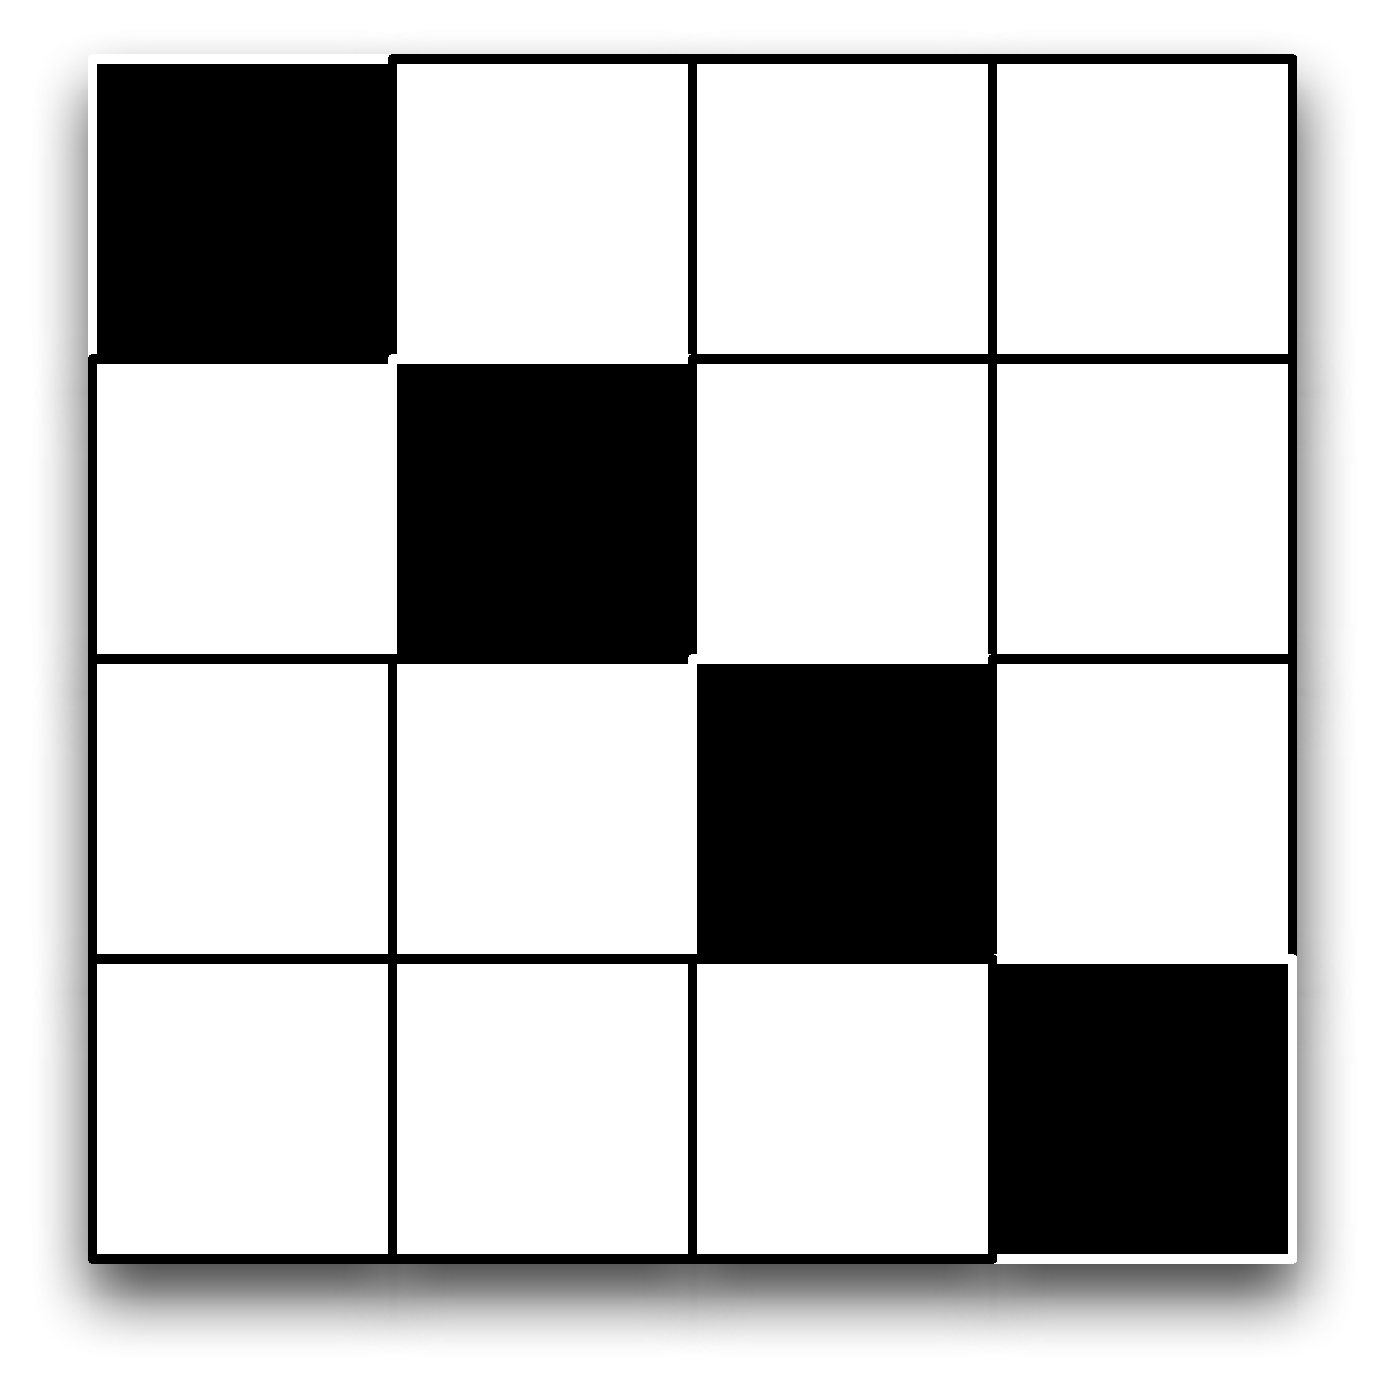
\includegraphics[width=1.5in]{Pictures/diag1.pdf}
\end{center}

\item
Give a Haskell function which takes an integer \texttt{n} and returns an  \texttt{n} by \texttt{n} white square with a diagonal black line from top right to bottom left, as in.
\begin{center}
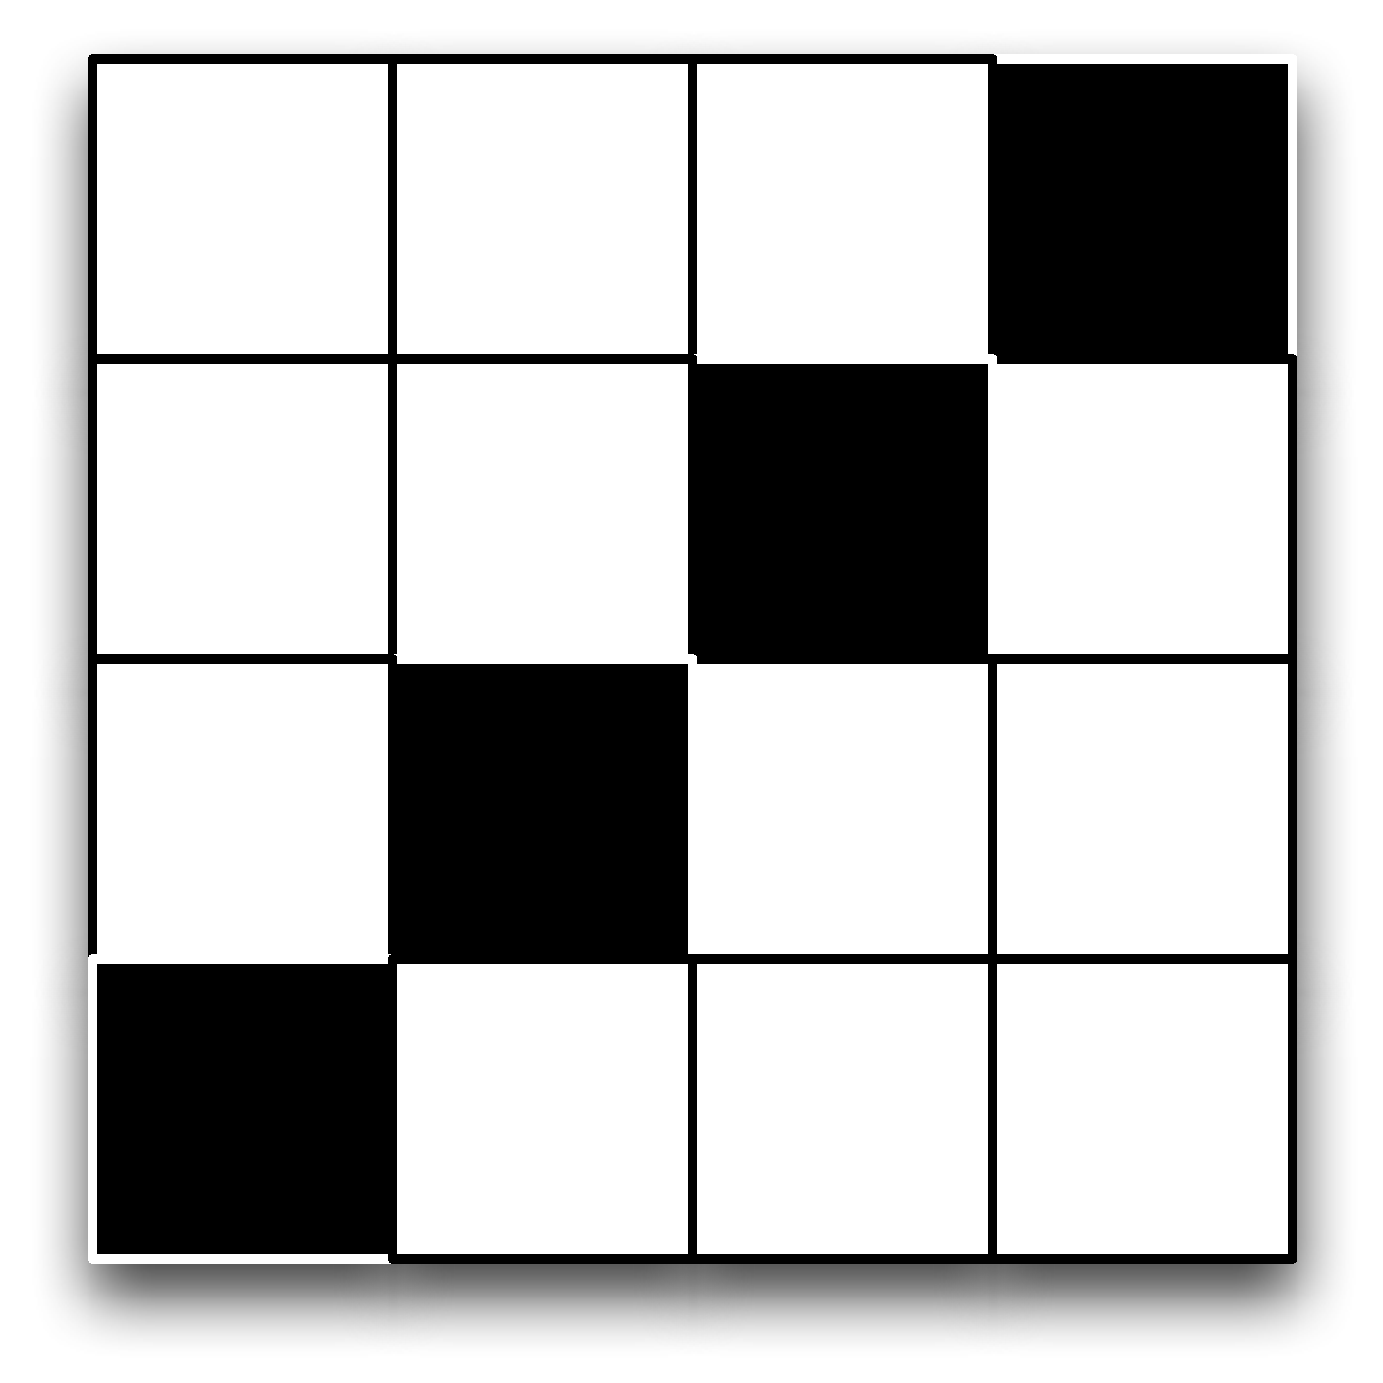
\includegraphics[width=1.5in]{Pictures/diag2.pdf}
\end{center}

\item
Give a Haskell function which takes an integer \texttt{n} and returns an  \texttt{n} by \texttt{n} white square with both diagonals coloured black, as in.
\begin{center}
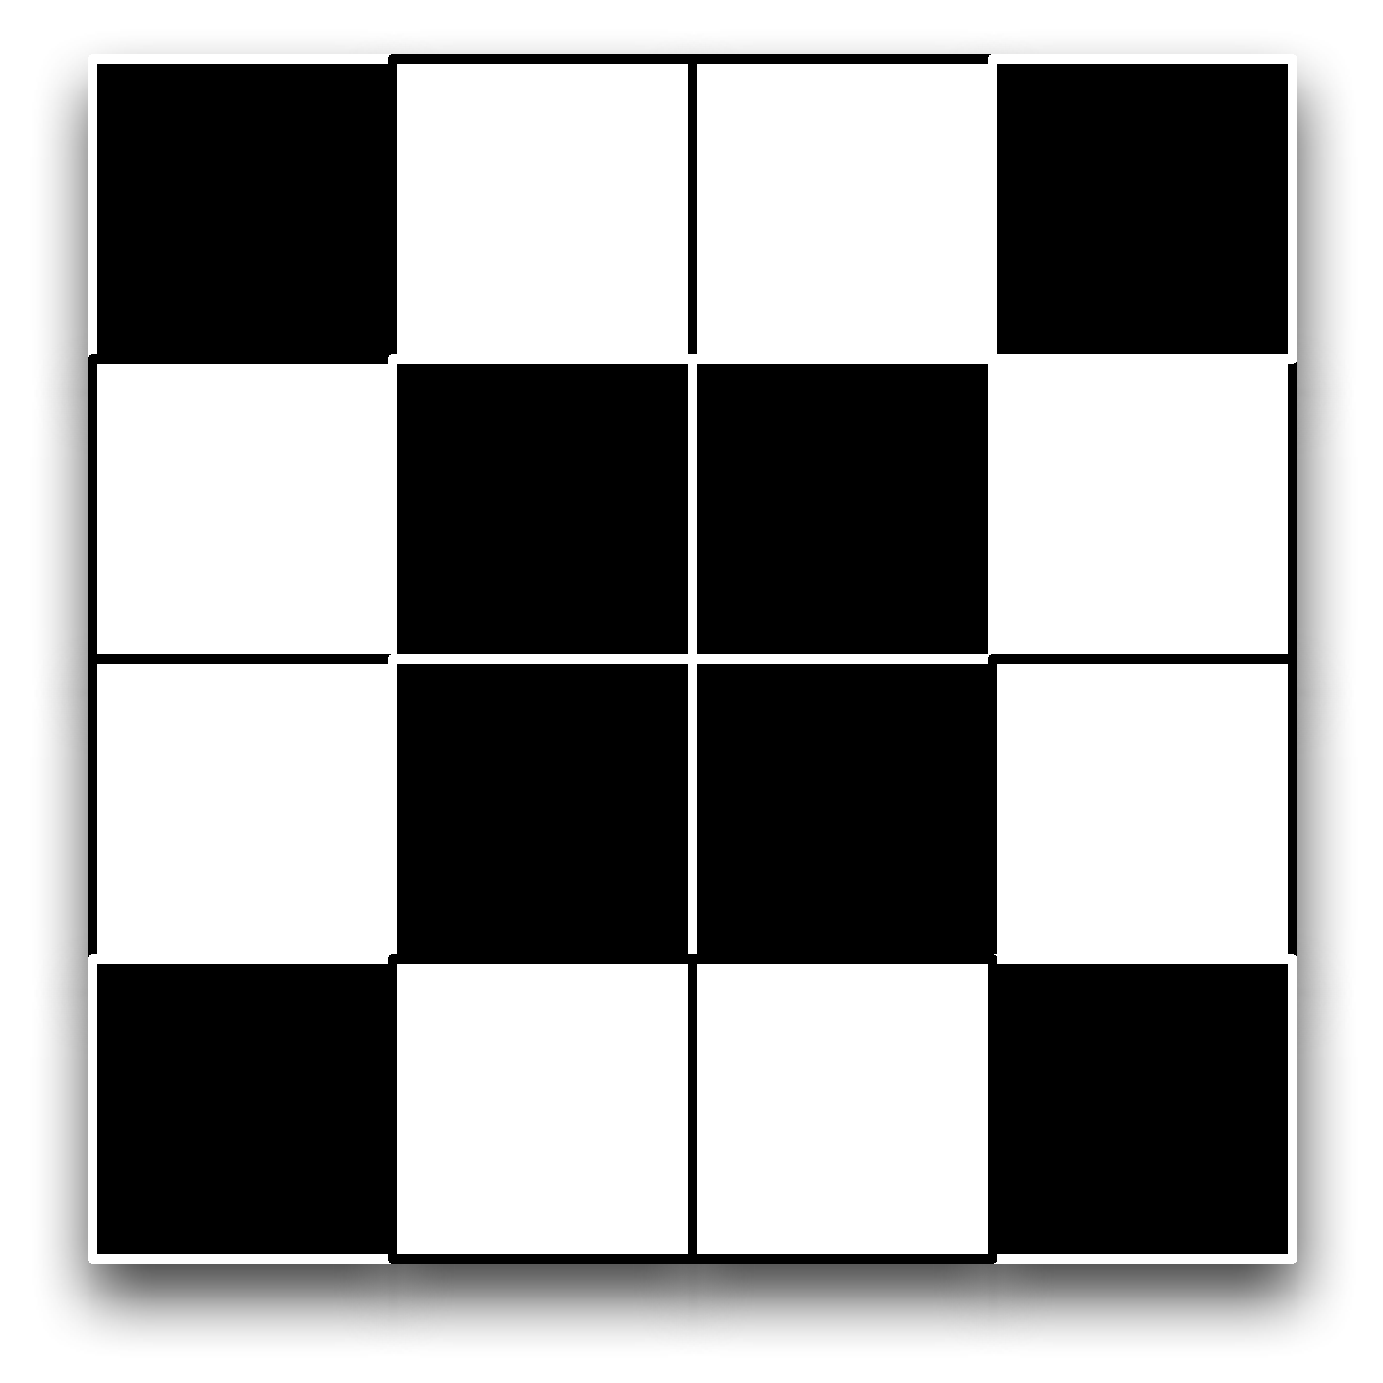
\includegraphics[width=1.5in]{Pictures/diag3.pdf}
\end{center}

\item
Can you give a direct recursive definition of a  function 
\begin{alltt}
chessBoard :: Integer -> Picture
\end{alltt}
so that 
\begin{alltt}
chessBoard n = ... chessBoard (n-1) ...
\end{alltt}
Hint: you might want to use some of the functions defined here, or variants of them, in writing your definition.

\end{exercises}

\index{pictures!extended exercise|)}



\section{General forms of recursion}
\label{genRecursion}
\index{general recursion|(}
\index{recursion!general|(}

As we explained  in Section \ref{recursionIntro}, a recursive
definition of a function such as \texttt{fac} would give the value of
\texttt{fac n}
using the value \texttt{fac (n-1)}. We saw there that \texttt{fac (n-1)}
is {\em simpler\/} in being closer to the base case \texttt{fac 0}. As
long as we preserve this property of becoming simpler, different patterns
of recursion are possible  and we look at some of them in this section.
These more general forms of recursion are called \textbf{general
recursion}.
In trying to use recursion to define a function we need to pose the
question:

\subsubsection*{In defining {\tt f n} which values of
{\tt f k} would help me to work out the answer?}

\begin{example}
\subexample*{1.}The sequence of Fibonacci numbers starts with
\texttt{0} and
\texttt{1},
\index{Fibonacci numbers}
and subsequent values are given by adding the last two values, so that
we get \texttt{0+1=1}, \texttt{1+1=2} and so forth. This can be given a
recursive definition as follows
\begin{alltt}
fib :: Integer -> Integer
fib n 
  | n==0        = 0
  | n==1        = 1
  | n>1         = fib (n-2) + fib (n-1)
\end{alltt}
where we see in the general case that \texttt{fib n} depends upon not
only \texttt{fib (n-1)} but also \texttt{fib (n-2)}.

This gives a clear description of the Fibonacci numbers, but
unfortunately it gives a very inefficient program for calculating them.
We can see that calculating \texttt{fib n} requires us to calculate both
\texttt{fib (n-2)} and \texttt{fib (n-1)}, and in calculating
\texttt{fib (n-1)} we will have to calculate \texttt{fib (n-2)}
{\em again}. We   look at ways of overcoming this problem in Section 5.2.

\subexample*{2.}Dividing one positive integer by another can be
done in many different ways. One of the simplest ways is
repeatedly to subtract the divisor from the number being
divided,  and we give a program doing that here. In fact we will
define two functions
\begin{alltt}
remainder :: Integer -> Integer -> Integer
divide    :: Integer -> Integer -> Integer
\end{alltt}
which separately give the division's remainder and quotient.

In trying to find a definition it often helps to look at an example.
Suppose we want to divide \texttt{37} by
\texttt{10}. We expect that
\begin{alltt}
remainder 37 10 = 7
divide    37 10 = 3
\end{alltt} 
If we subtract the divisor, \texttt{10}, from the number being divided, \texttt{37}, 
how are the values related?
\begin{alltt}
remainder 27 10 = 7
divide    27 10 = 2
\end{alltt}
The remainder is the same, and the result of the division is one less. 
What happens at the base case? An example is
\begin{alltt}
remainder 7 10 = 7
divide    7 10 = 0
\end{alltt} 
Using these examples as
a guide, we have
\begin{alltt}
remainder m n 
  | m<n         = m
  | otherwise   = remainder (m-n) n
\end{alltt}
\begin{alltt}
divide m n
  | m<n         = 0
  | otherwise   = 1 + divide (m-n) n
\end{alltt}
\end{example}

These definitions also illustrate another important point: a general recursive function
does not always give an answer; instead an evaluation may go on forever. 
Look at what happens if we evaluate
\begin{alltt}
remainder 7 0
\step remainder (7-0) 0
\step remainder 7 0
\step ....
\end{alltt} 
This calculation will loop for ever, and indeed we should expect problems
if we try to divide by zero! However, the problem also appears if we try to divide by a
negative number, for instance
\begin{alltt}
divide 4 (-4)
\step divide (4-(-4)) (-4)
\step divide 8 (-4)
\step ...
\end{alltt}
The lesson of this example is that in general there is no guarantee that a function defined
by recursion will always \textbf{terminate}.\index{termination} 
We will have termination if we use primitive 
recursion, and other cases where we are sure that we always go from a more 
complex case to a simpler one; the problem in the example here is that
subtracting a negative number increases the result, giving a more complex application of the
function.
\index{recursion|)}
\index{general recursion|)}
\index{recursion!general|)}


\begin{exercises}

\item
Give a recursive definition of a function to find the highest common
factor of two positive integers.

\item 
Suppose we have to raise \texttt{2} to the power \texttt{n}. If
\texttt{n} is even, \texttt{2*m} say, then
\begin{alltt}
\superscr{2}{n} = \superscr{2}{2*m} = \superscr{(\superscr{2}{m})}{2}
\end{alltt}
If \texttt{n} is odd, \texttt{2*m+1} say, then
\begin{alltt}
\superscr{2}{n} = \superscr{2}{2*m+1} = \superscr{(\superscr{2}{m})}{2}*2
\end{alltt}
Give a recursive function to compute
\superscr{2}{n} which uses these insights.
\end{exercises}


\section{Program testing}
\label{testing}
\index{testing|(}

Just because a program is accepted by the Haskell system, it does not
mean that it necessarily does what it should.
How can we be sure that a program behaves as it is intended to? One
option, first aired in Section \ref{proof}, is to \textbf{prove} in some way that
it behaves correctly. Proof is, however, an expensive business,
and we can get a good deal of assurance that our programs behave
correctly by testing the program. 

If we are not to use proof, then we can use \textbf{QuickCheck} to test properties of functions using randomly generated data. This has a number of advantages -- we don't have to select input data, for example -- but we do need to define the properties to be tested, and it is not always clear how to do this. So, we can also do traditional testing, where we specify the inputs and expected result for a function.

The art of testing
is then to choose the inputs to be as comprehensive as possible. That is, we
want to test data to represent all the different `kinds' of input that can be
presented to the function.

How might we choose
test data? There are two possible approaches. We could simply be told
the \textbf{specification}\index{specification} of the function, and
devise test data according to that. This is called \textbf{black box}
testing\index{testing!black box}, as we cannot see into the box which
contains the function. On the other hand, in devising \textbf{white box}
\index{testing!white box}tests we can use the form of the function
definition itself to guide our choice of test data. We will explore
these two in turn, by addressing the example of the function
which is to return the maximum of three integers,
\begin{alltt}\minx{maxThree}
maxThree :: Integer -> Integer -> Integer -> Integer
\end{alltt}
 
\subsection*{Black box testing}
\index{testing!black box}

How can we make a rational choice
of test data for a function, rather than simply picking (supposedly) random numbers out
of the air? 

What we need to do is try to partition the inputs into
different \textbf{testing groups}\index{testing!testing groups}
where we expect the function to behave in a similar way for
all the values in a given group. In picking the test data
we then want to make sure that we choose at least one
representative from each group. 

We should also pay particular attention to 
any \textbf{special cases},\index{testing!special cases} 
which will occur on the `boundaries' of the
groups. If we have groups of positive and negative numbers, then we
should pay particular attention to the zero case, for instance.

What are the testing groups for the example of \texttt{maxThree}? There
is not a single right answer to this, but we can think about what is likely
to be relevant to the problem  and what is likely to be irrelevant. In
the case of \texttt{maxThree} it is reasonable to think that the size or
sign of the integers will not be relevant: what will determine the
result is their relative ordering. We can make a first subdivision this
way
\begin{itemize}
\item all three values different;
\item all three values the same;
\item two items equal, the third different. In fact, this represents two
cases
\begin{itemize}
\item two values equal to the maximum, one other;
\item one value equal to the maximum, two others.
\end{itemize}
\end{itemize}
We can then pick a set of test data thus
\begin{alltt}
6 4 1
6 6 6
2 6 6
2 2 6
\end{alltt}
If we test our definition in Section \ref{guards} with these data then
we see that the program gives the right results. 

We can code these tests in the HUnit\minx{HUnit} unit testing framework, like this:
\begin{alltt}
testMax1 = TestCase (assertEqual "for: maxThree 6 4 1" 6 (maxThree 6 4 1))
testMax2 = TestCase (assertEqual "for: maxThree 6 6 6" 6 (maxThree 6 6 6))
testMax3 = TestCase (assertEqual "for: maxThree 2 6 6" 6 (maxThree 2 6 6))
testMax4 = TestCase (assertEqual "for: maxThree 2 2 6" 6 (maxThree 2 2 6))

-- To run the tests, type 
--   runTestTT testsMax\minx{runTestTT}

testsMax = TestList [testMax1, testMax2, testMax3, testMax4]
\end{alltt}
Let's look at what is going on here. The final line collects all the tests into a list, which allows us to run the tests in one go, as we see below. Each test case involves some `boilerplate' code, but the crucial parts are the three arguments to \texttt{assertEqual} (which says we're doing a test of two things being equal):
\begin{itemize}
\item 
A \texttt{String} printed in case the test fails, e.g. \texttt{"for:\ maxThree 6 4 1"}.\looseness=-1
\item
The \emph{expected result}, e.g. \texttt{6}.
\item
The \emph{expression we want to evaluate}, e.g. \texttt{maxThree 6 4 1}.
\end{itemize}
We can run the tests in GHCi like this: 
\begin{alltt}
\textsl{*Chapter4>} runTestTT testsMax
\textsl{Cases: 4  Tried: 4  Errors: 0  Failures: 0
Counts \{cases = 4, tried = 4, errors = 0, failures = 0\}}
\end{alltt}
The
following program also meets these tests:
\begin{alltt}\minx{mysteryMax}
mysteryMax :: Integer -> Integer -> Integer -> Integer
mysteryMax x y z
  | x > y \&\& x > z      = x
  | y > x \&\& y > z      = y
  | otherwise           = z
\end{alltt}
so should we conclude that \texttt{mysteryMax} computes the maximum of the
three inputs? If we do, we are wrong, for we have that
\begin{alltt}
mysteryMax 6 6 2 \step 2
\end{alltt}
If we add the following test case to the test set:
\begin{alltt}
testMax5 = TestCase (assertEqual "for: mysteryMax 6 6 2" 6 (mysteryMax 6 6 2))
testsMMax = TestList [testMMax1, testMMax2, testMMax3, testMMax4, testMMax5]
\end{alltt}
and run the tests, we get these results:
\begin{alltt}\index{testing!failing case}
\textsl{*Chapter4>} runTestTT testsMMax
\textsl{### Failure in: 4
for: mysteryMax 6 6 2
expected: 6
 but got: 2
Cases: 5  Tried: 5  Errors: 0  Failures: 1
Counts \{cases = 5, tried = 5, errors = 0, failures = 1\}}
\end{alltt}
This is an important example: it tells us that \textbf{testing alone
cannot assure us that a function is correct}. 
How might we have spotted this error in designing our test data? We
could have said that not only did we need to consider the groups above,
but that we should have looked at all the different possible orderings
of the data, giving
\begin{itemize}
\item all three values different: six different orderings;
\item all three values the same: one ordering;
\item two items equal, the third different. In each of the two cases we
consider three orderings.
\end{itemize}
The final case generates the test data \texttt{6 6 2} which find the
error.

We mentioned special cases earlier: we could see this case of two equal
to the maximum in this way. Clearly the author of \texttt{mysteryMax}
was thinking about the general case of three different values, 
so we can see the example as underlining the importance of
looking at special cases.

\subsection*{White box testing}
\index{testing!white box}

In writing white box test data we will be guided by the principles
which apply to black box testing, but we can also use the form of the
program to help us choose data.
\begin{itemize}
\item If we have a function containing guards, we should supply data
for each case in the definition. We should also pay attention to
`boundary conditions' by testing the equality case when a guard uses
\texttt{>=} or \texttt{>}, for example.
\item If a function uses recursion we should test the zero case, the one
case and the general case.
\end{itemize}
In the example of \texttt{mysteryMax} we should be guided to the data 
\texttt{6 6 2} since the first two inputs are at the boundaries of the
guards
\begin{alltt}
x > y \&\& x > z                       y > x \&\& y > z
\end{alltt}
We take up the ideas discussed in this section when we discuss proof in
Chapter \ref{reasoningProgs}.


\begin{figure}[t]\index{QuickCheck!\texttt{Int} and \texttt{Integer}}
\beware{QuickCheck with \texttt{Int} and \texttt{Integer}}{
Suppose we define 
\begin{alltt}
\ \ fact :: Int -> Int
  
\ \ fact n

\ \ \ \ | n>1       = n * fact (n-1)

\ \ \ \ | otherwise = 1
\end{alltt}
we would expect this property to be true whatever the input \texttt{n}:
\begin{alltt}
\ \ prop\_fact n =

\ \ \ \ fact n > 0
\end{alltt}
But if we try this out, we get this result
\begin{alltt}
\ \ \textsl{*Chapter4>} quickCheck prop\_fact

\ \ \textsl{*** Failed! Falsifiable (after 14 tests and 2 shrinks):    
17}
\end{alltt}
and we can see that this is indeed true:
\begin{alltt}
\ \ \textsl{*Chapter4>} fact 17

\ \ \textsl{-288522240}
\end{alltt}
This is because \texttt{Int} is a fixed-size representation of integers, and when numbers become big enough, they `wrap around' into the negative. 

\medskip
The lesson of this example is that if you expect the integers in your program to behave like the `real' integers, then you should use \texttt{Integer} rather than \texttt{Int}.
}
\end{figure}



\begin{exercises}

\item
Devise test data for a function
\begin{alltt}
allEqual :: Integer -> Integer -> Integer -> Bool
\end{alltt}
intended to test whether its three integer inputs are equal.

\item
Use the test data from the previous question to test the function
\begin{alltt}
solution m n p = ((m+n+p)==3*p)
\end{alltt}
Discuss your results.

\item
The function 
\begin{alltt}
allDifferent :: Integer -> Integer -> Integer -> Bool
\end{alltt}
should return \texttt{True} only if all its inputs are different. Devise
black box test data for this function.

\item
Test the following function
\begin{alltt}
attempt m n p = (m/=n) \&\& (n/=p)
\end{alltt}
using the test data written in the previous question. What do you
conclude on the basis of your results?

\item
Devise test data for a function
\begin{alltt}
howManyAboveAverage :: Integer -> Integer -> Integer -> Integer
\end{alltt}
which returns how many of its three integer inputs are larger than their
average value.

\item
Devise test data for a function to raise two to a positive integer
power.

\item
Repeat these exercises to define QuickCheck properties which can be used to test these functions.
\index{testing|)}
\end{exercises}

\begin{summary}
This chapter has introduced some general principles of program design.
\begin{itemize}
\item We should think about how best to use what we already know. If we
have already defined a function \texttt{f} we can make use of it in two ways.
\begin{itemize}
\item[--] We can {\em model\/} our new definition on the
definition of \texttt{f}.
\item[--] We can {\em use\/} \texttt{f} in our new definition.
\end{itemize}
\item We should think about how to break the problem into smaller, more
easily solved, parts. We should ask {\em What if I had ...?}.
\begin{itemize}
\item[--] This could be another function, which we can define separately.
\item[--] It could also be a local definition, defined in a \texttt{where} clause.
\end{itemize}
\item We can define \texttt{data} types to model our problem domain. We'll come back to this in later chapters, where we'll discover ways of building complex types from simpler ones, as well as how to define more complex \texttt{data} types.
\item We can use recursion to define functions.
\end{itemize}
We also explained the basics of recursion, and saw how it is used in
practice to define a variety of functions. We shall see many more
illustrations of this when we look at recursion over lists in Chapter 7.

We concluded by showing that it was possible to think in a principled
way about designing
test data for function definitions rather than simply choosing the first
data that came to mind.
 \end{summary}

%\end{document}
